% !TeX root = main.tex
% !TEX program = lualatex

\documentclass[11pt,a4paper]{article}	

\usepackage[T1]{fontenc}
\usepackage[english,polish]{babel}
\usepackage{csquotes}
\usepackage[style=numeric]{biblatex}
\usepackage{lipsum}
\usepackage{fontspec}
\setmainfont{Roboto}
\usepackage[table,usenames,dvipsnames]{xcolor}
\usepackage{hyperref}
\usepackage[bottom=3cm,marginparwidth=1.5cm, marginparsep=0.5cm]{geometry}
\geometry{a4paper}	
\usepackage{graphicx}
\usepackage{tikz}				
\usetikzlibrary{shapes,backgrounds,mindmap,trees}
\usepackage{wrapfig}
\usepackage{fancyhdr}
\usepackage{gensymb}
\usepackage{setspace}

\addbibresource{./bib/rethinking_resource_depletion.bib}
\addbibresource{./bib/limits_to_growth.bib}
\addbibresource{./bib/shaping_the_global_oil_peak.bib}
\addbibresource{./bib/ipcc2018.bib}
\addbibresource{./bib/global_climate_change.bib}
\addbibresource{./bib/renewable_review_2000.bib}
\addbibresource{./bib/renewable_problems.bib}
\addbibresource{./bib/first_fission_reactor.bib}
\addbibresource{./bib/fission_problems.bib}
\addbibresource{./bib/hybrid_nuclear_renewable.bib}
\addbibresource{./bib/fission_tech_and_current_issues.bib}
\addbibresource{./bib/structural_materials_fusion.bib}
\addbibresource{./bib/fusion_history.bib}
\addbibresource{./bib/nuclear_fusion_status.bib}
\addbibresource{./bib/fusion_fuel_running_out.bib}
\addbibresource{./bib/iter_website.bib}
\addbibresource{./bib/iter_timeline.bib}
\addbibresource{./bib/w7x_website.bib}
\addbibresource{./bib/fusion_records.bib}
\addbibresource{./bib/iter_delays.bib}
\addbibresource{./bib/iter_diagnostics_count.bib}
\addbibresource{./bib/iter_data_throughput.bib}
\addbibresource{./bib/iter_realtime_processing.bib}
\addbibresource{./bib/xilinx_what_is_fpga.bib}
\addbibresource{./bib/iter_re_melt.bib}
\addbibresource{./bib/massive_gas_injection.bib}
\addbibresource{./bib/hxrm_jet.bib}
\addbibresource{./bib/pmts_basics.bib}
\addbibresource{./bib/low_noise_amplifier_for_pmt.bib}
\addbibresource{./bib/why_pmt_need_amplifiers.bib}
\addbibresource{./bib/pmt_gain.bib}
\addbibresource{./bib/analog_vs_digital_1998.bib}
\addbibresource{./bib/mca_fpga.bib}
\addbibresource{./bib/dpp_walewski.bib}
\addbibresource{./bib/kstar_upgrade.bib}
\addbibresource{./bib/mwd.bib}

\onehalfspacing
\setlength{\parskip}{\baselineskip}%
\setlength{\parindent}{0pt}%
%============================================================================%
%	BEGIN DOCUMENT
%============================================================================%
\begin{document}
\selectlanguage{polish}
% print title
\begin{titlepage}



% Upper part of the page. The '~' is needed because \\
% only works if a paragraph has started.

\includegraphics[width=4.3cm]{media/unilogo.png}
\hspace{\fill}

\includegraphics[width=2cm]{media/faculty.jpg}

\begin{center}
Politechnika Łódzka\\% Title
Wydział Elektrotechniki, Elektroniki, Informatyki i Automatyki Politechniki Łódzkiej\\% Title
\end{center}
%CONTENT
\begin{center}




Praca Dyplomowa Magisterska
Real Time Digital Pulse Processing from Radiation Detectors Using Field Programmable Gate Arrays
inż. Wojciech Mateusz Walewski
Nr albumu: 239587

% Author and supervisor
\noindent
\begin{minipage}{0.8\textwidth}
\begin{flushright} \large
\emph{Promotor:} \\
dr hab. inż. Dariusz Makowski, prof. uczelni\\
\end{flushright}
\end{minipage}

\vfill


% Bottom of the page
{\today}




\vfill
\end{center}
\end{titlepage}


\newpage
\selectlanguage{english}

\tableofcontents
\newpage

\selectlanguage{polish}
\begin{abstract}

\lipsum[1-3]


\end{abstract}
\newpage

\selectlanguage{english}
\begin{abstract}

\lipsum[3-5]
\end{abstract}
\newpage

\section{Introduction}


\subsection{Motivation}
  Concerns regarding the sustainability of using fossil fuels for energy generation
  have been raised as early as the 1970s \cite{rethinking_resource_depletion}. 
  One of the most well-known examples from that time was the 1972 report
  titled "Limits to Growth" by Meadows et. al. \cite{limits_to_growth}.
  In it a group of MIT scientists attempted to answer the question of
  how long will the Earth's natural resources last for
  considering the seemingly neverending growth of human civilisation.
  As a result of a conducted computer simulation,
  a rough estimate of around 100 years was given as a timeframe,
  after which the population would start to collapse due to a lack of resources.


  This estimate did not go without controversies back when it was first published.
  The methodology was thoroughly picked apart,
  leading many to dismiss the study findings
  \cite{rethinking_resource_depletion}.
  Naturally, nowadays, we are much better poised to verify
  the claims made by the now 50 year old book. The impeding resource depletion
  has certainly been made a less valid claim as technological progress
  made it possible to locate and tap into
  previously inaccesible fossil fuel fields
  \cite{shaping_the_global_oil_peak}.
  Taking into account other issues, however, 
  the original timeline of 100 years might have
  actually shifted closer. 


  When it comes to fossil fuel usage, in the last twenty years, 
  the primary concerns have changed from resource depletion to global warming 
  and irreversible environmental damage \cite{rethinking_resource_depletion}.
  In 2018 the Intergovermental Panel on Climate Change (IPCC) published a
  report indicating the need to stop the global temperature increase 
  at 1.5\degree C above the levels measurable in the pre-industrial era.
  Failure to do so is projected to lead to irreversible climate changes
  and in turn serious damage to human settlements around the world.
  \cite{ipcc2018}


  Fossil fuels account for as much as 70\% of greenhouse gas emissions.
  Electricity generation alone causes 25-35\% 
  \cite{global_climate_change} of the total amount.
  Such a high share means that reducing this output
  is going to be crucial in meeting the goals outlined by the IPCC.
  At the beginning of the twentieth century, renewable energies, i.e. 
  wind, solar, biomass and geothermal were thought
  to be the perfect solution to the issue at hand
  \cite{renewable_review_2000}. 


  In modern times, we have now become aware of multiple issues
  that make renewable energy generation a problem at large scale.
  Most importantly, their efficacy varies depending on the geographical
  location and climate. Even when placed in optimal conditions,
  they do not offer perfect stability. Additionally, the land
  usage is greater than the traditional forms of energy production
  \cite{renewable_problems}.

\subsection{Fission energy}

  The drawbacks of renewable energies have led to a formation
  of an alternative approach in both research and policymaking. 
  The use of nuclear energy for supplementing the shortcomings 
  of renewables has been suggested as a potential path forward.
  This concept is referred to as hybrid nuclear-renewable system.
  \cite{hybrid_nuclear_renewable}. 

  There are two ways that nuclear energy can be created and harnessed.
  In the more well-established technology, fission, heavy atoms 
  (usually Uranium) are bombarded with neutrons 
  and split into two or more lighter nuclei and
  additional neutrons as shown in \autoref{fig:fission}.
  The reaction is self-sustaining 
  and releases energy in the form of heat that is then used
  to boil water. The steam causes turbines to spin
  and generate electricity.
	\begin{figure}[H]
	  \centering
	  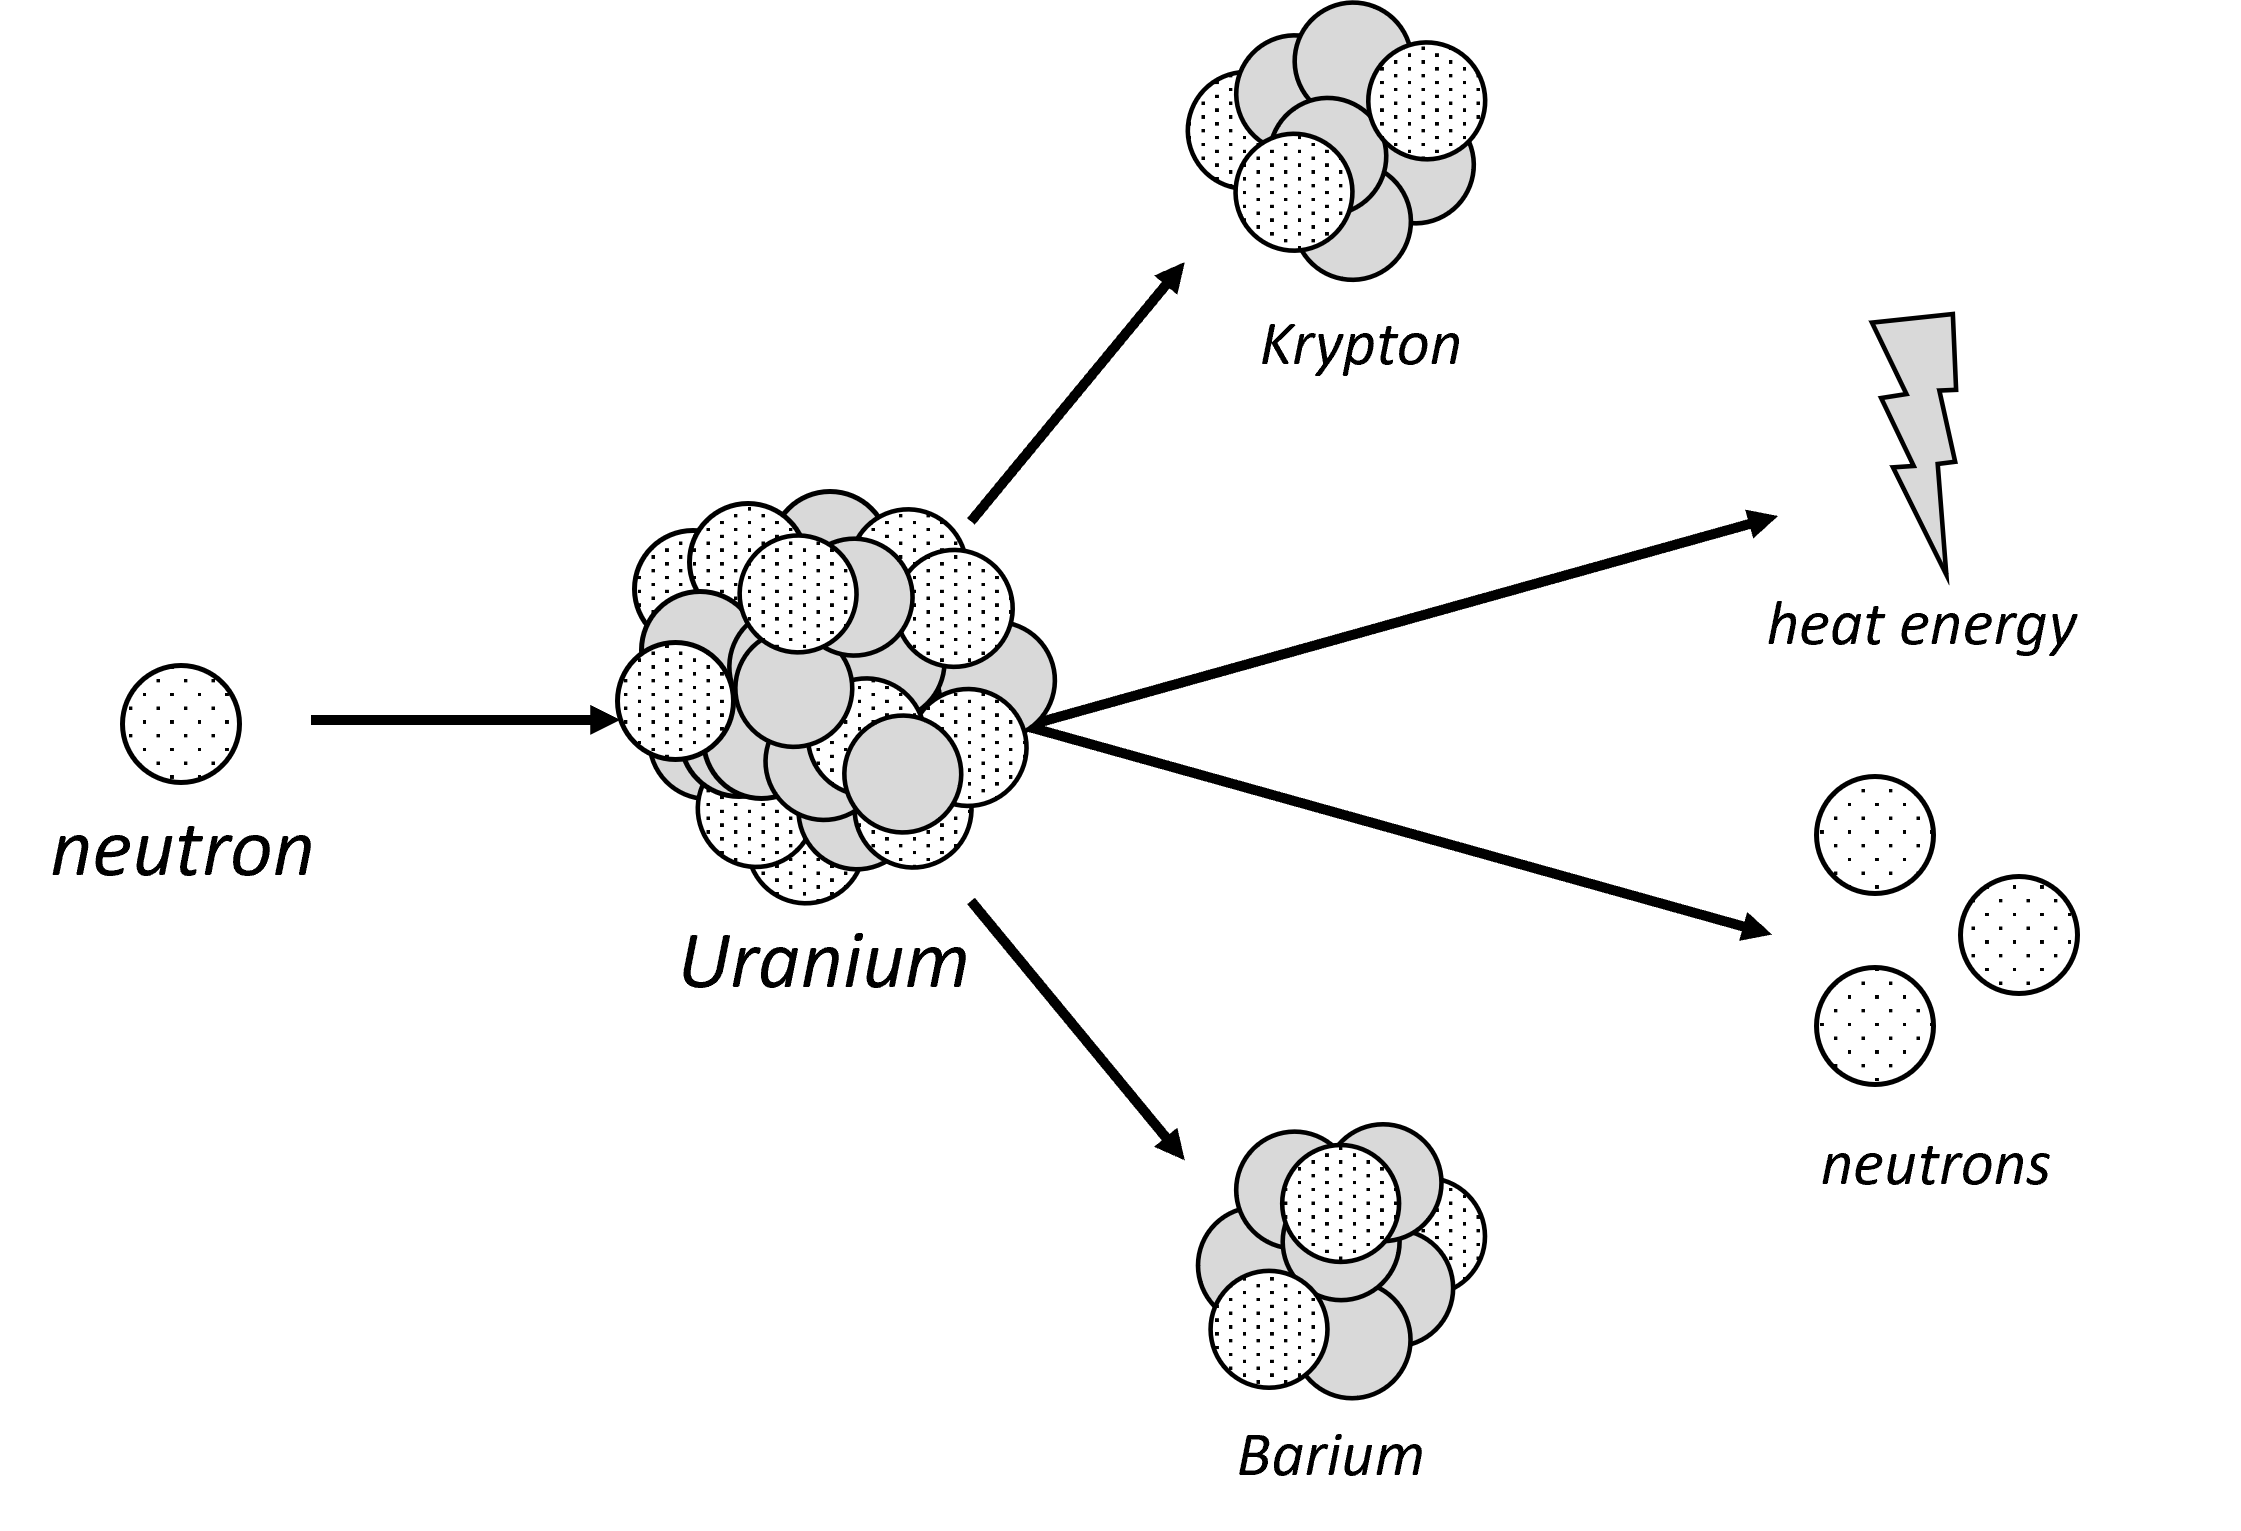
\includegraphics[width=.75\linewidth]{media/fission.png}
	  \caption{Uranium fission reaction}
	  \label{fig:fission}
	\end{figure}

  Fission is far from a new concept, as first fission reactors have been 
  built as early as 1942 \cite{first_fission_reactor}. 
  Although the technology itself is quite old 
  and has been greatly improved over time, 
  there is reasonable reluctance to build and use fission power plants. 
  The issue that gets raised most often is the storage of radioactive waste. 
  There are, however, multiple less well-known
  problems with fission \cite{fission_problems}. 


  The tragedies of Chornobyl and Fukushima reactors
  have caused many people to be wary of fission. However, even if
  democratic support is disregarded in policymaking, the acquisition,
  storage and disposal of radioactive materials required for and produced 
  during fission prove to be an administrative challenge, especially 
  if reactor construction and maintenance is to be handled
  by private entities \cite{fission_tech_and_current_issues}. 
  The complexity of the problem suggests that 
  as we arrive to more concrete solutions we 
  should not stop exploring other potential alternatives.

\subsection{Fusion energy}

  Just like it is possible to split atoms, it is also possible to
  combine them together in a process referred to as fusion. 
  Fusing atoms lighter than Iron is a reaction that 
  can produce surplus energy as highlighted by \autoref{fig:binding_energy}.
  Two atoms of low binding energy can fuse into an atom of higher 
  binding energy, releasing heat based on the mass-energy equivalence formula.
  The output energy can be used to generate electricity in
  the exact same manner as with fission. 
  The problem with fusion reactors is that the conditions necessary
  for fusion to happen are extremely harder to achieve and sustain 
  \cite{structural_materials_fusion}.
	\begin{figure}[H]
	  \centering
	  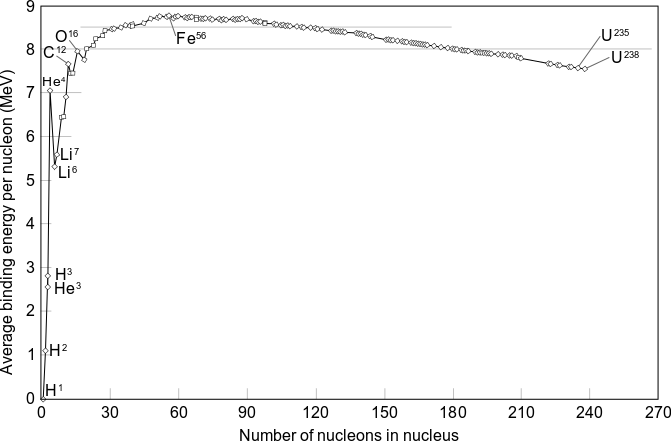
\includegraphics[width=.85\linewidth]{media/binding_energy.png}
	  \caption{Average binding energy per nucleon as a function of the number of nucleons in the atom}
	  \label{fig:binding_energy}
	\end{figure}

  Fusion is the primary reaction that causes stars to emit light and heat.
  The reaction that is most often artificially attempted on Earth differs
  from that occurring naturally in the Sun. There, a p-p reaction occurs. 
  This means the need of converting 4 protons into ${}^{4}$He.
  Replicating this reaction on a larger scale is extremely challenging 
  due to the need to convert protons into neutrons.
  On Earth, fusion experiments primarily rely on using hydrogen isotopes, 
  most commonly deuterium (D) and tritium (T) shown in \autoref{fig:fusion}.
	\begin{figure}[H]
	  \centering
	  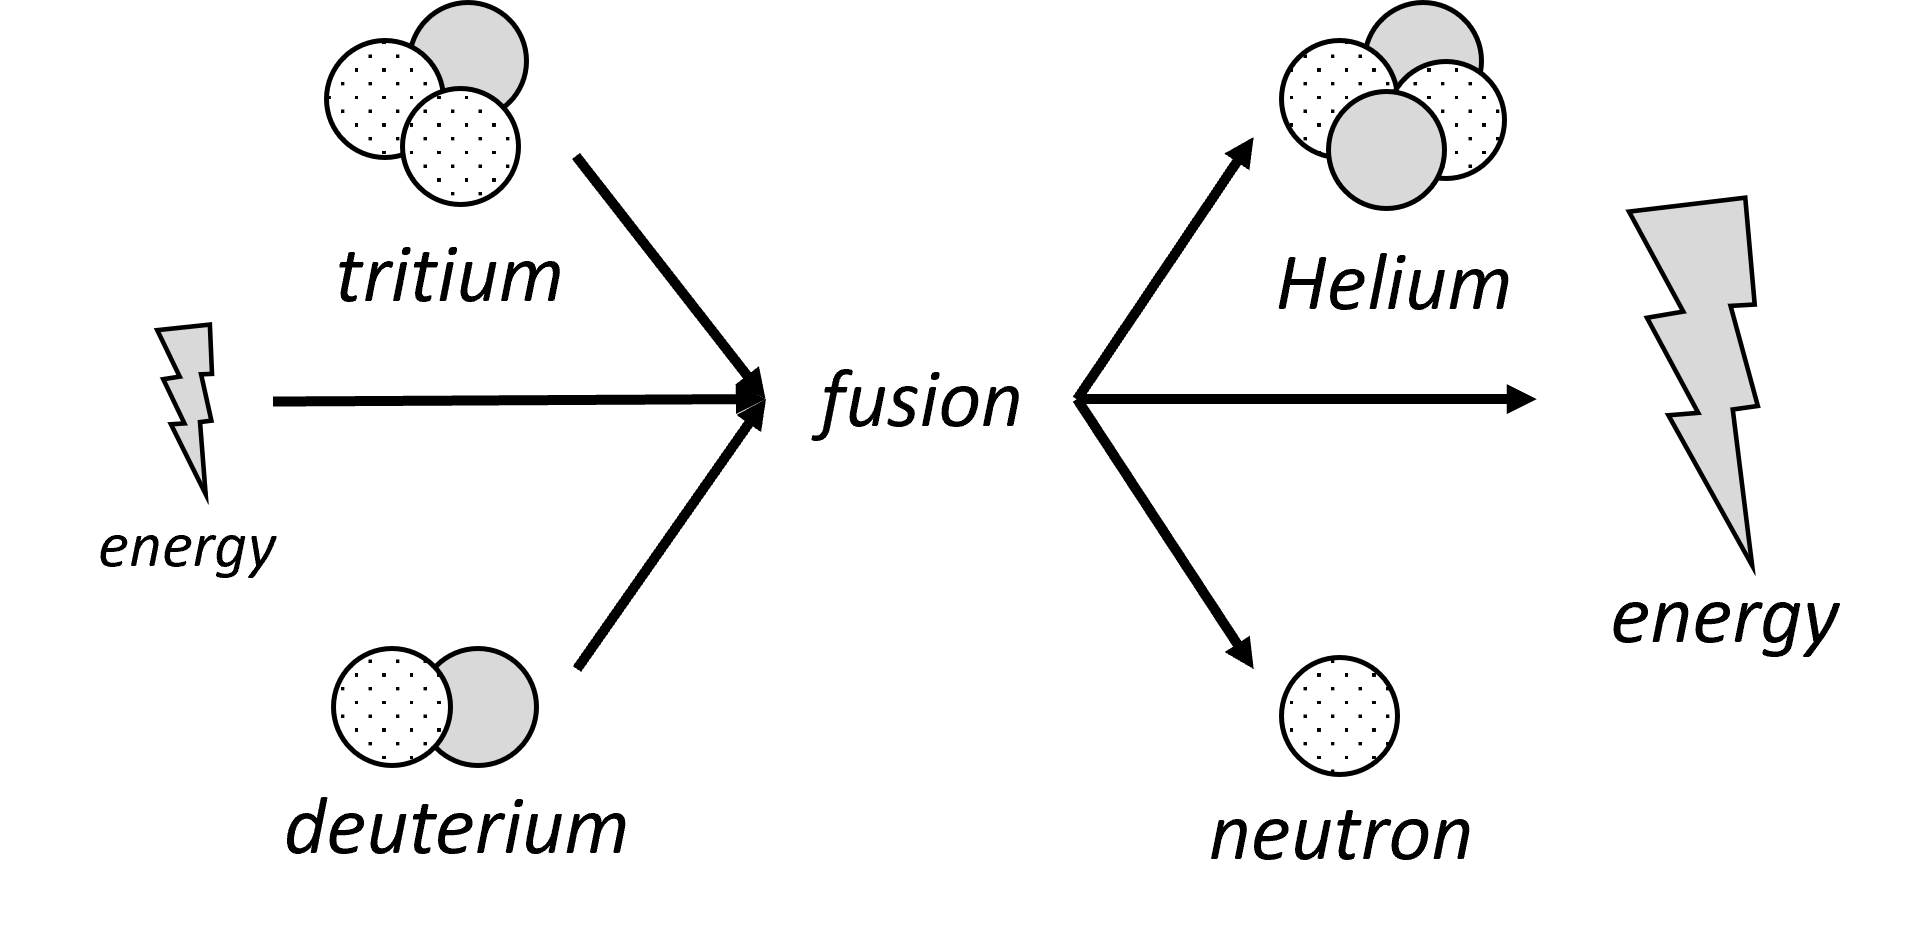
\includegraphics[width=.75\linewidth]{media/fusion.png}
	  \caption{D-T fusion reaction}
	  \label{fig:fusion}
	\end{figure}



  Despite being an easier approach, it still requires us to sustain
  a 200 million \degree C plasma. This means that an enormous amount of energy
  must be used to first heat the plasma up and then confine it to 
  prevent it from completely destroying the reactor. 
  The efficiency of D-T reactions might, however, worth the trouble.
  Theoretically, just 30 mg of deuterium would generate as much energy
  as 250 l of gasoline \cite{nuclear_fusion_status}. 


  Such numbers sound incredible, but there are naturally multiple drawbacks too.
  Tritium, the other input material of this most promising reaction is
  extremely rare in nature. Its artificial production is currently 
  done only by a select number of facilities. 
  Combined with its relatively short half-life of around 12 years, 
  there are fears of it running out. It is proven that fusion reactors
  will be capable of "breeding" their own tritium, however the transition period 
  may still prove to be troublesome \cite{fusion_fuel_running_out}.


  In the end, despite being a similarly old technology as fission
  \cite{fusion_history},
  a fusion reactor with a net positive energy balance
  has not yet been constructed. Containing plasma heated to such extreme
  temperatures cannot be achieved with any solid material and must 
  be done with the use of inertial or magnetic forces. 
  The most common reactors that employ this concept are:
  tokamaks (\autoref{fig:iter_reactor}) 
  and stellarators (\autoref{fig:w7x_reactor}).
  The former design has been selected for probably
  the most ambitious fusion project to date, 
  the International Thermonuclear Experimental Reactor (ITER)
  \cite{nuclear_fusion_status}.

  \begin{figure}[H]
    \centering
    \begin{minipage}{.5\textwidth}
      \centering
      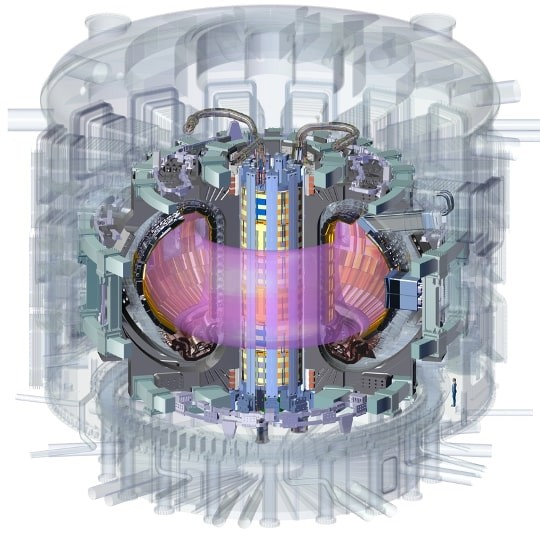
\includegraphics[width=.5\linewidth]{media/iter_reactor_3d.jpeg}
      \caption{ITER tokamak model\cite{iter_website}}
      \label{fig:iter_reactor}
    \end{minipage}%
    \begin{minipage}{.5\textwidth}
      \centering
	  \includegraphics[width=.65\linewidth]{media/w7x_3d.png}
      \caption{Wendelstein W7X sterellator model\cite{w7x_website}}
      \label{fig:w7x_reactor}
    \end{minipage}
  \end{figure}

\subsection{ITER Tokamak Project}
  \subsubsection{Tokamak}
	\begin{figure}[H]
	  \centering
	  \includegraphics[width=.75\linewidth]{media/iter_crosssection.jpeg}
	  \caption{ITER tokamak cross section\cite{iter_website}}
	  \label{fig:iter_crosssection}
	\end{figure}
	Tokamaks are reactors composed of a toroidal vacuum chamber surrounded by
	massive electromagnetic coils as shown in \autoref{fig:iter_crosssection}.
	The magnetic fields are used to shape plasma 
	and keep it away from the device internal walls. 
	Operation starts with the removal of air and impurities from the vessel.
	The gaseous fuel is introduced and a strong current is induced 
	ionizing the gases, thus forming plasma. Additional heat is introduced with
	microwave and fuel injections. Particles within the
	formed plasma can then collide with such force that they begin
	to break through atomic repulsion and fuse producing a large amount of energy.
	\cite{iter_website}
  \subsubsection{ITER Goals}

	At 24 m height and 30 m width, 
	ITER will be the biggest tokamak ever constructed. 
	That's twice as big as the largest experimental reactor currently in service, 
	the Joint European Torus (JET). JET has been working since 1983 with 
	a goal of achieving net energy gain. Despite running successful 
	plasma experiments and recently starting deuterium-tritium experiments,
	the highest fusion energy gain Q 
	(the ratio of produced power to the power required to sustain the plasma)
	obtained by JET was 0.33. A record only recently topped by a different 
	type of a fusion device held at the US Department of Energy’s
	National Ignition Facility. Using laser technology it was possible to
	obtain a Q of 0.7 for 4 billionths of a second. \cite{fusion_records}
	

	Although not supposed to work as a power plant, just an experiment,
	throughout its operation ITER intends to break this record by a lot.
	The new reactor is designed to reach an energy gain of 10 
	for the duration of a few minutes. This is of course still a theoretical
	plan, as the facility is still a fairly long time from being finished.
	As of 2022, the vacuum vessel is yet to be welded together\cite{iter_timeline}.
	First plasma operation is scheduled for the end of 2025\cite{iter_timeline},
	although multiple delays have already happened in the past \cite{iter_delays},
	so future ones would at this point not be too surprising. 
  \autoref{fig:iter_aerial} shows an aerial picture of ITER from 14th of April 2020.
  Not all facilities have been fully constructed at this time.
	\begin{figure}[H]
	  \centering
	  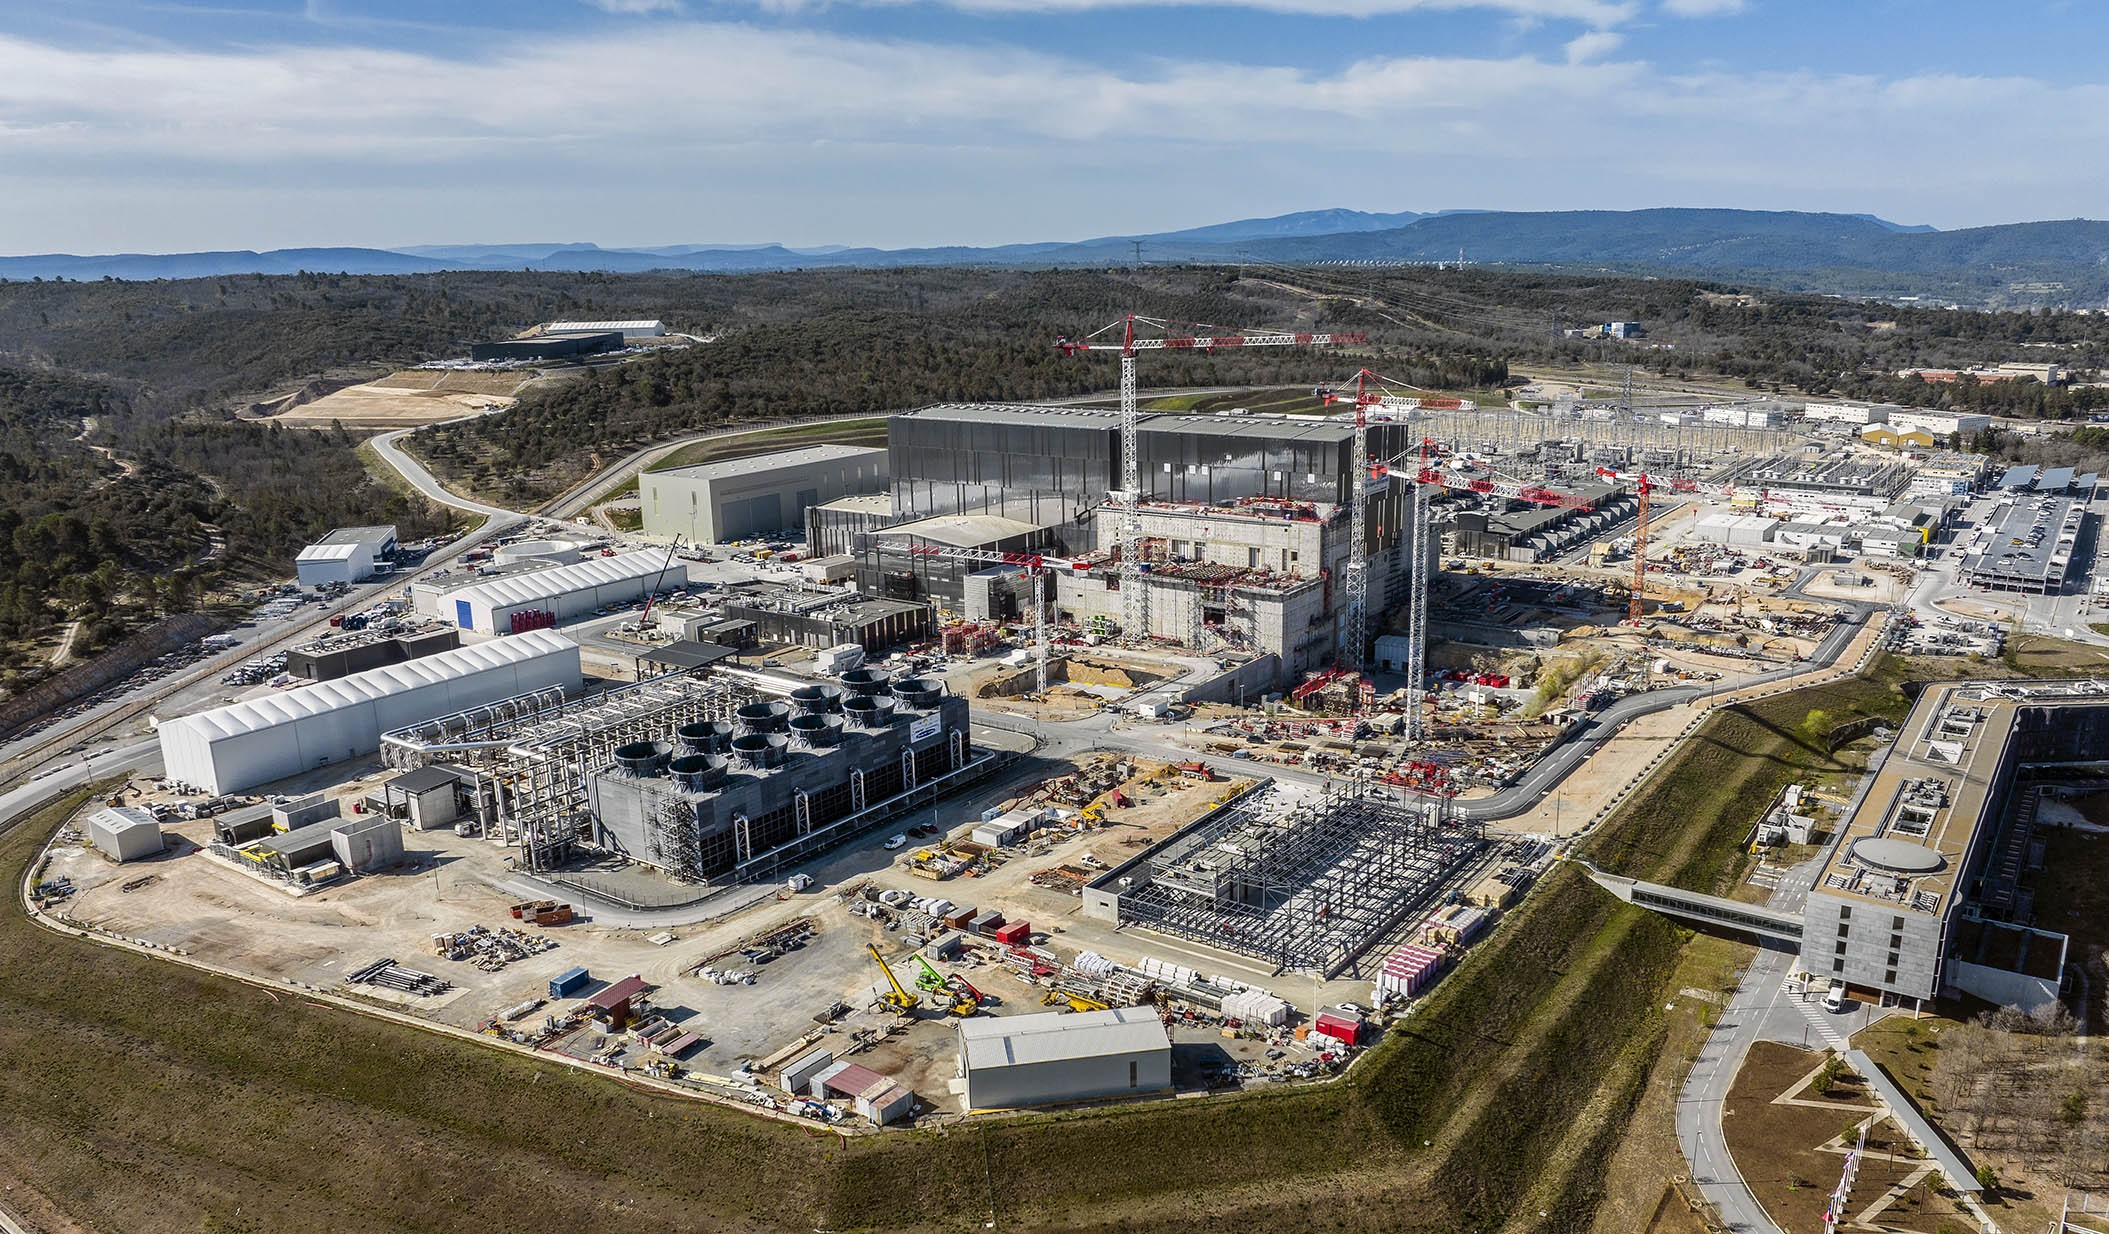
\includegraphics[width=.9\linewidth]{media/iter_aerial_2022.jpg}
	  \caption{Aerial view of the ITER facility as of 2022\cite{iter_website}}
	  \label{fig:iter_aerial}
	\end{figure}
	\subsubsection{Primary Concerns}

	With a project of this magnitude it is near impossible to predict
	everything that might go wrong. There are naturally safety concerns,
	questions regarding the ambitious goals set by the management and
	the troubles of international cooperation\cite{iter_delays}.
	It is thus crucial to maintain maximum operational safety 
	and log all experimental data. This should ensure that even in the 
	case of partial failure of the project important practical knowledge
	can be recorded for future fusion experiments.


	When operational, ITER will rely on around 50 completely different
	measurement systems to control, evaluate and investigate its plasma 
	\cite{iter_diagnostics_count}.
	This translates into dozens of gigabytes of data being generated, 
	processed and archived every second as the experiment is running 
	\cite{iter_data_throughput}.
	With some of the experiments lasting fractions of a second,
	a lot of the critical data acquisition and control must occur
	in real time and without waiting for human reaction 
	\cite{iter_realtime_processing}.
	This poses an important challenge when it comes to the choice
	of computing apparatus. A perfect device would offer
	infinite configurability preferably with remote access 
	as well as a very high data throughput. 

	Traditional computers or more precisely Central Processing Units (CPUs) 
	are remotely reprogrammable but may offer insufficient speeds in 
	some of the real time applications. On the other end of this scale lie 
	Application Specific Integrated Circuits (ASIC). These devices are an 
	arrangement of digital logic gates realizing one specific goal, like 
	digital signal filtering or processing network packets.
	ASICs offer unmatched bandwidth but cannot really be reconfigured
	after deployment, making them a risky choice in highly experimental
	applications such as tokamaks.

\subsection{Field Programmable Gate Arrays}
Devices that offer a compromise between speed and reconfigurability
exist nowadays. Most commonly Field Programmable Gate Arrays (FPGAs) are used.
FPGAs are formed out of matrices of so called Configurable Logic Blocks (CLBs).
These are small circuits that produce a single bit of logic output
out of 4 input bits, using a reprogrammable function. These blocks 
are then wired together using programmable interconnects. Such design 
allows for the implementation of very efficient digital algorithms
directly with the use of logical gates, without the need for an
entire processor. \cite{xilinx_what_is_fpga}


The interconnects and CLB internal structure introduce additional wiring
that would be unnecessary in the case of ASICs. These stray capacitances 
and inductances limit the maximum clock speed of FPGAs. This not too much
of an issue provided that the function can be parallelised. To offset 
this limitation, most FPGAs manufactured today come packed with 
more complex sub-circuitry that can be intermixed with the CLBs
as indicated in \autoref{fig:fpga_structure}.
These components can vary greatly from fast arithmetical blocks
to small CPU-based microcontrollers.

	\begin{figure}[H]
	  \centering
	  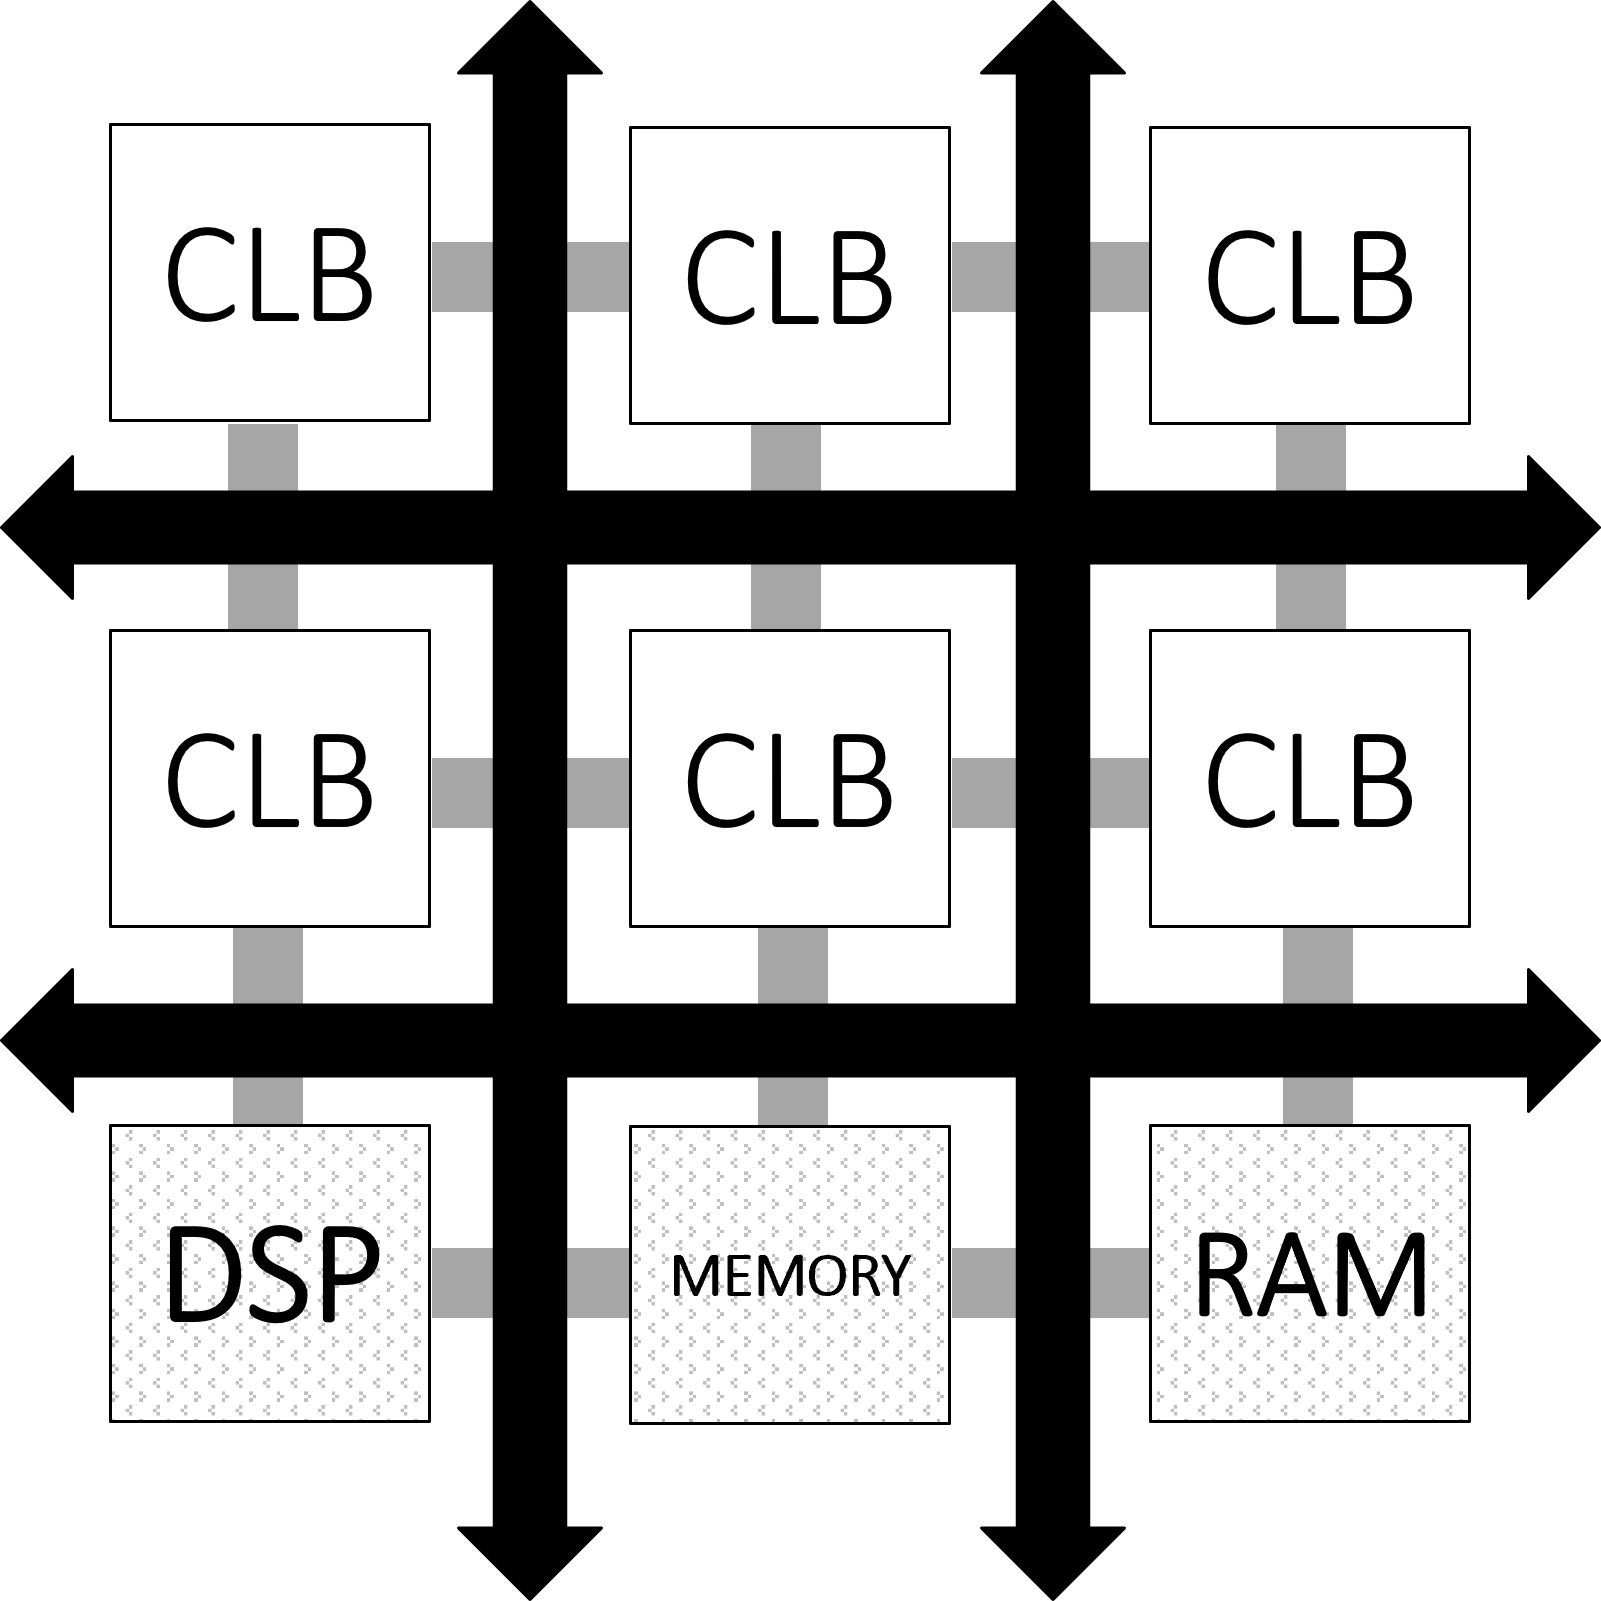
\includegraphics[width=.6\linewidth]{media/fpga_structure.png}
	  \caption{The internal structure of an FPGA}
	  \label{fig:fpga_structure}
	\end{figure}
\subsection{Problem statement}

The nature of FPGAs makes them instrumental in the data acquisition 
and control systems of modern fusion experiments like the ITER tokamak.
This work evaluates the potential usage of Field Programmable Gate Arrays
for the detection and analysis of pulses produced by PhotoMultiplier Tubes (PMTs)
being part of a High X-Ray Monitor (HXRM) designed to monitor Runaway Electorns
(REs) at tokamaks.


A functional system for the Digital Pulse Processing (DPP) at the rate of 
1 GS/s is proposed and implemented in an FPGA. A custom
software package for control and data acquisition is shown.
The optimization of both hardware and software is described.
Different algorithms for pulse detection and discrimination
are analysed, simulated and implemented in hardware. Finally design
considerations for future systems are given.


\newpage
\section{Hard X-Ray spectroscopy}

One of the diagnostic systems in a lot of currently existing tokamaks
is the Hard X-Ray Monitor (HXRM). It will also be implemented in ITER.
The device is tasked with measuring the spectrum of X-Ray radiation
inside the fusion vessel. The presence of high energy X-Ray
radiation can point to problems with the plasma stability and suggest the 
need for mitigation techniques.
\cite{low_noise_amplifier_for_pmt}

\subsection{Runaway electrons}

The plasma in a tokamak is heated to a level where particles reach a velocity
enabling them to break through atomic repulsion. In such conditions some 
particles can also obtain sufficient speed to escape the magnetic confinement
of the vessel. Typically collisions with other particles are so frequent
that in stable plasma these disturbances are not happening in large quantities.
Directly after plasma is disrupted or terminated, 
the probability of collisions is lessened 
and a tokamak might start acting like a particle accelerator,
bringing the electrons to nearly the speed of light.
Electrons that act in this manner are called Runaway Electrons (REs).
\cite{iter_re_melt}


This phenomenon can occur in the form of a high-energy 
concentrated beam capable of melting the front-facing walls of a reactor.
The effects of such damage being purposefully introduced in the JET tokamak
are shown in \autoref{fig:re_melt}. To prevent mitigate the destructive
effects of REs their generation has to be avoided if possible. Otherwise
they must be detected and dealt with accordingly. One method of doing so 
involves the injection of noble gases in a process called 
Massive Gas Injection (MGI) \cite{massive_gas_injection}.
\begin{figure}
  \centering
  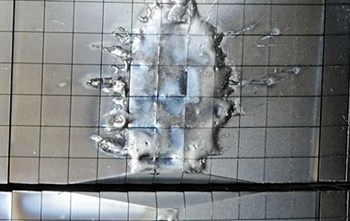
\includegraphics[width=.7\linewidth]{media/re_melt.jpeg}
  \caption{Effects of RE in the JET vessel\cite{iter_re_melt}}
  \label{fig:re_melt}
\end{figure}


When REs interact with the Plasma Facing Components (PFCs)
they lose their energy and emit X-Ray radiation in 
the Bremsstrahlung process. The energy of this radiation
varies greatly, ranging from tens of keV (Soft X-Ray)
to multiple MeV (Hard X-Ray).
\cite{hxrm_jet}

\subsection{PhotoMultiplier Tubes}

The photons generated in Bremsstrahlung by Runaway Electrons
can be detected with the use of a device known as a PhotoMultiplier Tube (PMT).
A PMT is built with the use of a photocathode and an electron multiplier.
When a radiation photon hits the photocathode an electron is emitted
due to the photoelectric effect. Electric fields in the PMT accelerate the 
electron towards a series of dynodes. Each collision with a dynode causes
a release of additional electrons and forms a stronger beam that 
eventually reaches the anode where it becomes measurable as a current pulse.
Typically a gain in the order of $10^6$ is obtained.
\cite{pmts_basics, pmt_gain}

\subsection{Preamplifiers}

The internal gain of a PMT is sufficient for many applications and 
does not require additional amplification. The produced current impulses 
can be detected with precise circuitry,
however there are multiple reasons for which
a preamplifier is often used in tangent with a PMT. With a typical
load of $50 \Omega$ the output signal of a single photon is
a very sharp voltage peak of around 10 mV.
Unprocessed short PMT pulses are sufficient for detection, counting 
and timing, but may be problematic when it comes to discrimination and 
processes like Pulse Height Analysis (PHA).
\cite{why_pmt_need_amplifiers}


In those scenarios that do not require the sharpest response,
the slight increase in Signal to Noise Ratio is worth the 
features introduced by an amplifier. These can include
impedance matching, filtering and pulse-shaping.
In tokamak applications it also helps move most of the 
diagnostic infrastructure away from the dangerous environment
created by the fusion plasma. 


In ITER the X-Ray radiation will first be converted to a light pulse
using a scintillator. This light will be transferred over a 12 m 
fiber before reaching the PMT. Then the electrical signal from 
the PMT must pass through a 100 m copper coaxial cable, before
reaching the acquisition and processing hardware. The internal 
input of a PMT is thus insufficient in this scenario and must be 
preamplified.
\cite{low_noise_amplifier_for_pmt}

\subsection{Pulse processing chains}

To obtain a radiation spectrum from the voltage pulses,
their height must be measured and
placed into an appropriate bin consisting of a range of voltage levels.
The pulses generated by a PMT last just a few nanoseconds,
making the task at hand complicated.


With a preamplifier this duration is increased by a factor of around
a few hundreds depending on the preamplifier components.
This results in pulses that last a few hundreds nanoseconds.
Before the advent of ultra-high speed Analogue to Digital Converters (ADCs),
such short events could not viably be processed with digital 
electronics and had to rely on analogue components.

\subsubsection{Analogue processing chains}

In analogue radiation spectroscopy
pulses are typically first transformed to a Gaussian shape,
with a series of low- and high-pass filters.
These signals must then pass through complicated pile-up
rejection circuitry. After that the pulses 
are fed to a Multi Channel Analyzer (MCA).
This is the device that performs the binning action.
Initially an MCA would consist of an array of 
analogue comparators, and over time it would rely 
on more and more digital components.


As mentioned earlier, for a long time analogue processing 
was the only way to reliably handle events shorter than 100 ns. 
It was, however, quickly recognized
that the digital approach offered 
much lesser susceptibility to outside noise. 
Digital components could also potentially be tuned without
having to physically modify the circuit.
These two features are particularly important in the 
complicated environment of a fusion reactor.
\cite{analog_vs_digital_1998}

\subsubsection{Digital processing chains}

As soon as ADCs and digital processing circuits capable of
reaching the resolution required for precise nuclear
spectroscopy appeared on the market they were 
adopted into new experimental designs of MCAs \cite{mca_fpga}.
As the technology improved ADCs were moved closer to the 
radiation detector itself.
A single reprogrammable silicon chip, together with a fast ADC,
could perform the job of a number of the analogue components
in a spectroscopy system.
On top of that its operation is less susceptible to Electro Magnetic
Interference (EMI) and temperature-induced parameter variance.
\cite{dpp_walewski}


The earlier in a processing chain that the ADC is placed the
lesser the influence of imperfect analogue components is.
Seeing an ADC right after the preamplifier is commonplace
in modern systems. Such approach, however, produces an important issue.
To obtain a sufficient horizontal resolution comparable to analogue chains
the ADC must sample the signal with a frequency of at least
a few hundred MHz. This means that, at a typical vertical resolution
of anywhere between 8 to 16 bits, a modern high-speed ADC
can generate anywhere between 100 megabytes 
up to even a few gigabytes of data every second.
\cite{dpp_walewski}


Processing gigabytes of data in real time poses one of 
the primary challenges in designing Digital Pulse Processing systems.
Despite that, fast digitizers are used for Hard X-Ray Spectroscopy
in existing tokamaks, like KSTAR or JET \cite{hxrm_jet, kstar_upgrade}.
ITER will require similar or better systems during its operation,
so the problems of handling large data throughput
should be considered solved before the diagnostic systems
are installed in the facility. Once first plasma is obtained,
the possibility of system modifications will be greatly limited.
 



\newpage
\section{System requirements}

The Hard X-Ray Monitor system must provide a real-time 
spectrum of the radiation produced by Runaway Electrons.

\newpage
\section{Research setup}
An FPGA powered data acquisition board was used as the platform 
for the hardware implementation of digital pulse processing of PMT
signals.
The following subsections describe the system component in detail and
\autoref{fig:system_overview} shows an overview of the testbench.
\subsection{PMT}
\subsection{Preamplifier}
\subsection{Digitizer board}
To acquire and digitize the signals produced by the PMT and preamplifier
combination Teledyne SP Devices ADQ14-4C was used. The board was connected
through PCIe 2.0 to the host PC running custom acquisition software.
ADQ14-4C can sample signals from up to 4 channels, each at a maximum
frequency of 1 GHz. 
\begin{table}[ht]
\caption{Chosen parameters of ADQ14-4C}
\centering
  \begin{tabular}{l l}
    material  & T [K]\\
    \hline
    Sn                     & 3,7 \\
    Pb                     & 7,2 \\
    Al                     & 1,2\\
  \end{tabular}
  \label{tab:adq14_datasheet}
\end{table}


The ADQ14 acquires samples with a 14-bit ADC.
The device applies factory calibrated digital gain and shift
to the raw measurements, 
so in order to maintain higher precision the samples are 
extended to 16 bits representing two full bytes. 
The additional two bits represent the fractional part potentially
produced by the fractional gain component.


The ADQ14 can operate in both triggered streaming and continuous mode.
In continuous mode samples are constantly gathered and periodically
transferred to the host PC. In triggered streaming a window of samples is 
collected only after a trigger event is detected. This is a basic feature
that allows for some data reduction, as only events of interest have to
be transferred to the host PC. Multiple triggering mechanisms, 
like level, periodic and external are available.


In all modes of operation the device relies on an internal 2 GB DRAM
to act as a FIFO queue for the generated records.
The device relies on Direct Memory Access (DMA) to transfer
data to the host PC. This is a special mode of operation for 
peripheral devices in which a chunk of the computer's memory is
made available to them without the need of CPU brokerage.


Unfortunately the maximum size of DMA buffers is limited. 
With a sampling speed of a 1 GHz and 2 byte samples up 
to two gigabytes of data can be generated each second for each
channel that is active. Even with reliance on DMA maintaining 
a transfer speed this high is problematic. The ADQ14's internal DRAM
acts as a buffer whenever the throughput becomes to high.
Records are first stored in the internal DRAM and periodically
transferred to the host PC's RAM whenever buffers become ready.

\subsubsection{Open FPGA design}

A crucial feature of ADQ14 is the fact that its core processing
functionality is realised with the use of an on-board FPGA,
more specificaly a Xilinx Kintex 7 K325T. The design of the FPGA
is partially open. Users can implement custom
filtering or data analysis on samples in real time.
This fact is used to implement the custom pulse processing described in this work.


The firmware is unfortunately not entirely open-source.
Third-party IP cores cannot be distributed to end customers 
and thus user algorithms are limited to two sections called User Logics.
User Logic 1 is a core placed after the ADC samples are subjected to factory
gain, but before the signals are passed on to trigger control.
This enables the implementation of custom triggering logic.


User Logic 2 is intended to house more complicated logic.
This module has access to the GPIO ports and some metadata
outputs, that can be used to better describe the transferred records.
User Logic 2 is located right before the encrypted packet generator
that is responsible for queueing the incoming data in ADQ14's DRAM 
for transfer to the host PC. The packet generator can be partially
controlled from within User Logic 2. Arbitrary data can be injected
in place of the samples for each channel and the size of transferred windows 
can be modified.

\subsubsection{Parallel sampling}

The FPGA is clocked only at 250 MHz which is exactly a quarter of 
the ADC maximum operating frequency. This means that each channel
of the digitizer outputs 4 samples on each clock cycle of the 
FPGA. This is a necessary design choice as FPGAs fare better 
at lower clock speeds due to the need of less complex routing
when it comes to connecting the various peripherals and CLBs.


Such design does however complicate the implementation of 
Digital Signal Processing. It is especially cumbersome for 
functions that depend on delayed samples.
Accumulators have the need of summing up 4 samples on
each clock cycle instead of one. Complicated operations
like multiplication and division require duplicated logic.
Most functionality must be properly pipelined to avoid
timing issues in the FPGA design.

\subsection{Host computer}
\subsection{Software package}
To control the acquisition process and handle the data transfer,
a custom software GUI application was developed. The application
employs an API provided by SP Devices to interface to the digitizer board.
The Qt5 framework is used for GUI display and multiple other functions.
The application leverages the Qt's signal/slot system heavily to synchronize
threaded events.


The primary thread of the software application
is used for UI display and general tasks like 
loading and saving configurations. A secondary thread
is spawned to control data acquisition and archival.
The proper operation of the secondary worker thread
is crucial in obtaining a high data throughput and 
the process of software optimization is described in 
CHAPTERDATATRANSFER

\newpage
\section{Pulse detection}
The prerequisite to any pulse processing is their detection. 
The window of interest containing a pulse to be analysed
must be properly distinguished from the surrounding noise.
Although detection is a must, it also brings the added benefit
of data rate reduction. If pulses can be accurately 
marked within a signal it is possible to transfer only
those samples that compose the events. 


The ADQ14 is capable of sampling signals with a frequency of
up to 1 GHz. With two bytes per sample, a single channel 
generates 2 GBs of raw data per second. For the PCIe 2.0 interface,
that is used in this work, the manufacturer's 
datasheet specifies a theoretical maximum throughput of 3.2 GB/s.
Even if this perfect limit could be obtained it would not allow 
for two channels to be active at once.
Using pulse detection for data reduction is thus unavoidable.
It is crucial to use a robust algorithm for this process to ensure 
that almost no pulses go unnoticed and near to none
false positives are transmitted.

\subsection{Level trigger}
The most basic approach to detection is a level trigger,
a technology available to any spectroscope. As shown in 
\autoref{fig:level_trigger}, a trigger occurs when
the input signal crosses a predefined voltage level,
either on a rising or a falling edge. The point at which
this occurs marks the beginning of a record window.
In the simplest case the end of a window is placed
a fixed duration from the start.


Once a window finishes, no more events are detected
until the signal returns to a value below the trigger level
(for rising edge triggering). This reset value might be 
set to be equal to the trigger level, however such approach
might lead to a scenario shown in \autoref{fig:lt_no_hysteresis}.
In a noisy environment the signal might falsely trigger immediately after
a window ends due to a random high spike on the slower falling edge of
an exponential pulse.


To prevent such false triggers typically some form of a hysteresis is used.
The reset level is shifted downwards, so that the input signal must cross
such a threshold that the random noise is almost guaranteed to never cause false 
triggers. \autoref{fig:lt_hysteresis} shows a hysteresis mitigating some false triggers.


With the slow falling edge of a pulse care must be taken not to 
overestimate the hysteresis. By setting the reset level too far away
from the trigger level pile-ups can be missed as pointed to in
\autoref{fig:lt_hysteresis_overshoot}. With a properly set hysteresis
the level trigger offers performance that is sufficient in most applications,
as suggested by its prevalence in modern spectroscopes.
In a tokamak's environment, however, the hysteresis
alone could potentially prove insufficient due to 
electromagnetic and temperature fluctuations having an effect on noise.

\subsection{Boxcar filter}

The two problems most apparent to simple level triggering 
are its susceptibility to noise and pulse overlap.
Just as with analogue approaches these two problems 
can be minimized with low-pass and high-pass filtering.
By utilizing a low-pass filter the input signal becomes 
smoother and more averaged, reducing the possibility of 
false triggers caused by random spikes. A high-pass filter
would reduce the DC component of the falling edge of a pulse,
making pile-ups easier to detect.


In the digital domain the simplest filters that perform
these operations are the Moving Average (MA) filter and 
the derivative filter. MA works to reduce the spikes and increase 
SNR. The derivative filter can strip the DC component from
a signal, meaning that the sharp rising edges will become
more attenuated in comparison to the decaying tails.


By combining the concepts of the MA and derivative filters
into a single a Boxcar filter is obtained. An example transfer
function of a Boxcar filter is shown in \autoref{fig:boxcar_transient}.
The effect of the filter on an example exponential pulse are shown 
in \autoref{fig:boxcar_effect}. The filter can be considered
to be a subtraction of two samples averaged with a window
of length $W$ delayed from each other by $W$.



\subsection{Trapezoidal filter}
\subsection{Triangular filter}
\subsection{Other solutions}
\subsection{Simulation performance}
\subsection{Hardware implementation}
\subsubsection{Boxcar filter}
\subsubsection{Trapezoidal filter}
\subsubsection{Triangular filter}

\newpage
\section{Pulse Height Analysis}
\subsection{Pulse shaping algorithms}
\subsection{Integration}
\subsection{Hardware implementation}
\newpage
\section{Data transfer} \label{sec:data_transfer}

The ADQ14's datasheet specifies a maximum data rate of 3.2 GB/s 
with the PCIe interface. The board is sold with a PCIe 2.0 x8 
interface which has a theoretical throughput of 4 GB/s.
The datasheet figure is thus likely an estimate placed at 80\% of 
the maximum or a best case scenario benchmark. In a real system 
the multitude of configuration options makes reaching this value
complicated. ADQ14 merges all data transferred from its internal DRAM 
to the PC into a single stream, so the data transfer must be 
optimized to the highest degree.
\autoref{fig:acquisition_buffers} shows an overview
of the data transfer process at different stages.

\begin{figure}[H]
  \centering
  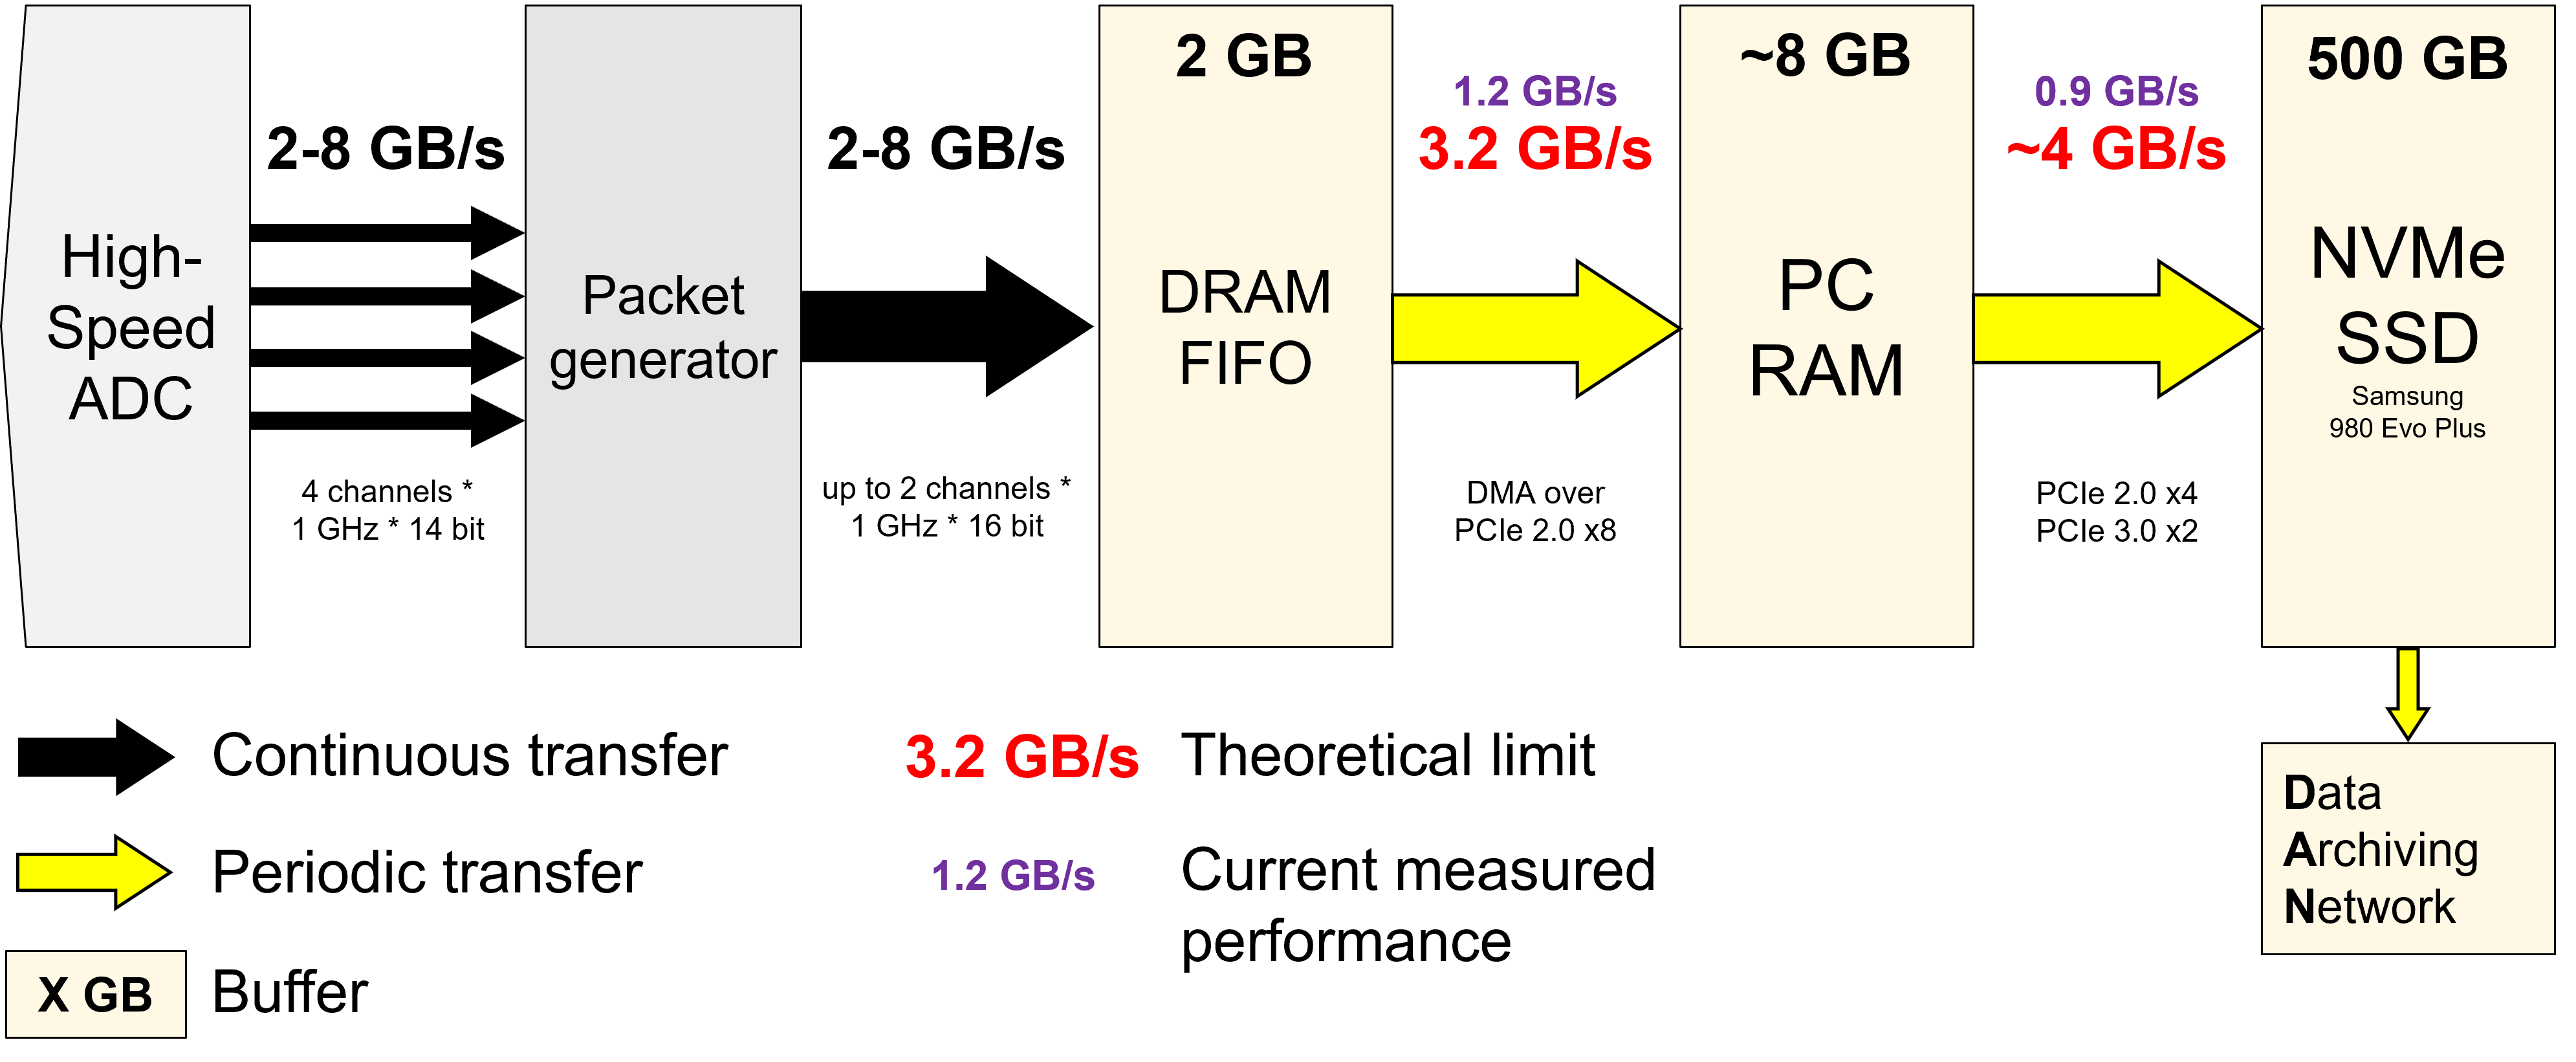
\includegraphics[width=\linewidth]{media/acquisition_buffers.png}
  \caption{Data transfer in the system}
  \label{fig:acquisition_buffers} 
\end{figure}

\subsection{PCIe interface}

A first point that can be considered for improvement is the hardware interface itself.
As of 2022 PCIe 4.0 is supported by both major CPU manufacturers.
Newest Intel processors can also make use of the PCIe 5.0 standard, 
with AMD devices to follow suit in the near future.
By upgrading the digitizer board to support PCIe 3.0 in the same x8 configuration the
theoretical throughput would double to 8 GB/s. With PCIe 4.0 it would become 16 GB/s.
Naturally, this is an issue that lies completely on the side of the board's manufacturer.
Future digitizer boards might need to target more modern interconnection standards,
to provide throughput necessary for ultra-high-speed signal acquisition.

\subsection{Direct memory access}

When using DMA, the ADQ14 splits the outgoing data into buffers.
The number and size of the buffers is configurable. Depending
on the desired application different settings should be preferred. 
To verify how the DMA buffer configuration affects transfer speed a simple
test was developed. The digitizer was programmatically configured with 
a series of varying buffer sizes and counts and used to run 20 
acquisitions, each 10 seconds long. The acquired data was not 
saved to disk, only copied in RAM.

\autoref{fig:buffer_size_speed} and \autoref{fig:buffer_count_speed}
show how the average throughput changes depending on the
configuration. In the tests with a varying buffer size 16 transfer buffers were used.
When testing the influence of the buffers count on the throughput,
the buffer size was set to 65536 bytes.
Generally larger buffers, or a higher count of buffers
provide better maximum throughput up to a certain maximum.
Increasing the size of buffers seems to provide a more consistent improvement. 
  \begin{figure}[H]
    \centering
    \begin{minipage}{.45\textwidth}
      \centering
      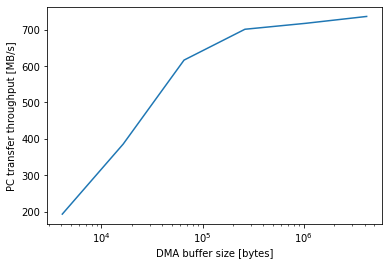
\includegraphics[width=\linewidth]{media/buffer_size_speed.png}
      \caption{DMA buffer size influencing the transfer throughput}
      \label{fig:buffer_size_speed}
    \end{minipage}%
    \hfill
    \begin{minipage}{.45\textwidth}
      \centering
      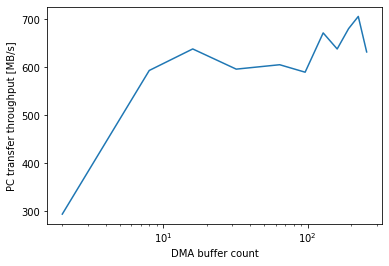
\includegraphics[width=\linewidth]{media/buffer_count_speed.png}
      \caption{DMA buffer count influencing the transfer throughput}
      \label{fig:buffer_count_speed}
    \end{minipage}
  \end{figure}

Larger buffer sizes unfortunately mean that records are packed together
into larger pages. The first record of a page will be transferred
with a significant delay in relation to its occurrence.
For example, with a record length of 1024 and a buffer size capable
of holding 10240 samples, after an event occurs, 9 more events
would have to get recorded for the first one to get transferred to the PC.


ITER's specification requires a maximum of a 5 ms delay when it comes
to transferring the acquired data to the Plasma Control System.
If the same digitizer board will also have to transfer the raw
samples for archiving and offline analysis, care will have to 
be taken when configuring these parameters. Transferring the raw signal
will require a considerable amount of bandwidth, suggesting the need for a larger
buffer size. At the same time whenever a spectrum window is finished
it should be transferred to the PC as soon as possible.
Buffers no larger than a single spectrum would work best for that.
Most likely a compromise will have to be reached experimentally.

\subsection{Developed acquisition software}

To control the acquisition process and handle the DMA data transfers,
a custom software GUI application was developed. The application
uses an API provided by SP Devices to interface with the digitizer board,
but implements a custom processing routine and algorithms.
The Qt5 framework is used for GUI display and multiple other features.
Most importantly, the application leverages the Qt's signal/slot system 
to synchronize threaded events.


First prototypes of the application were developed with the use of PyQt, 
a library with Qt5 framework bindings for Python.
As the scope of the application grew
and the need for finer control over the performance became a priority,
the application was ported over to C++ and developed further.
\autoref{fig:qtadqscope_v1}, \autoref{fig:qtadqscope_v2} and
\autoref{fig:qtadqscope_v3} show how the application's UI 
changed with major releases.

\begin{figure}[H]
  \centering
  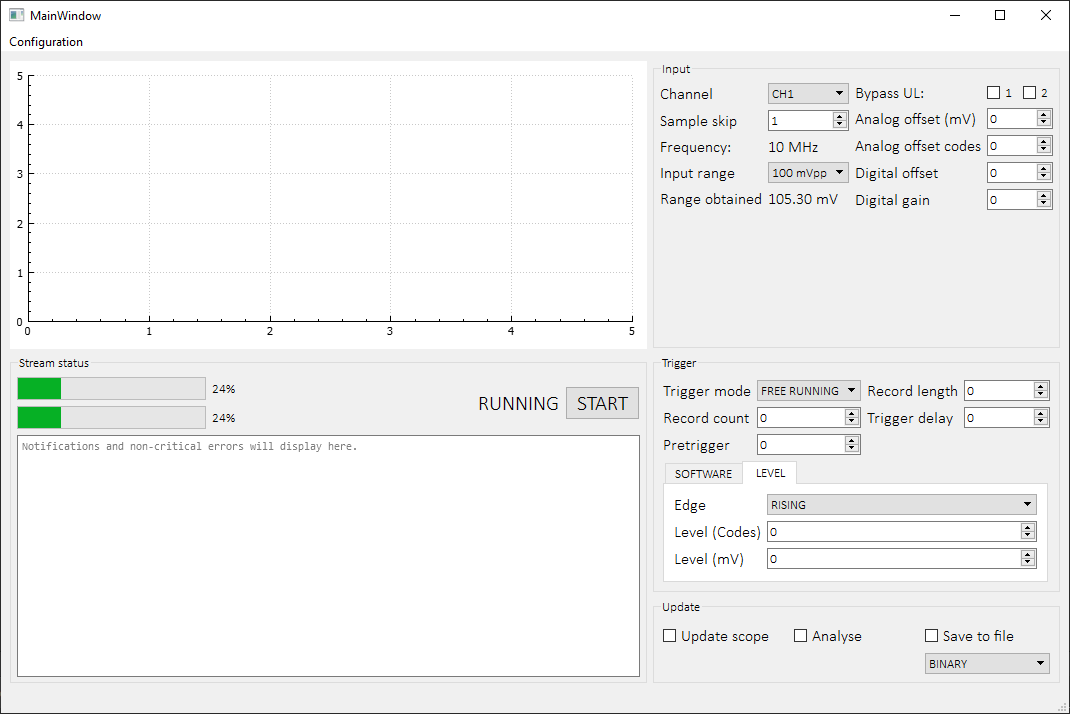
\includegraphics[width=\linewidth]{media/qtadqscope_v1.png}
  \caption{First functional acquisition software GUI written in C++}
  \label{fig:qtadqscope_v1} 
\end{figure}
\begin{figure}[H]
  \centering
  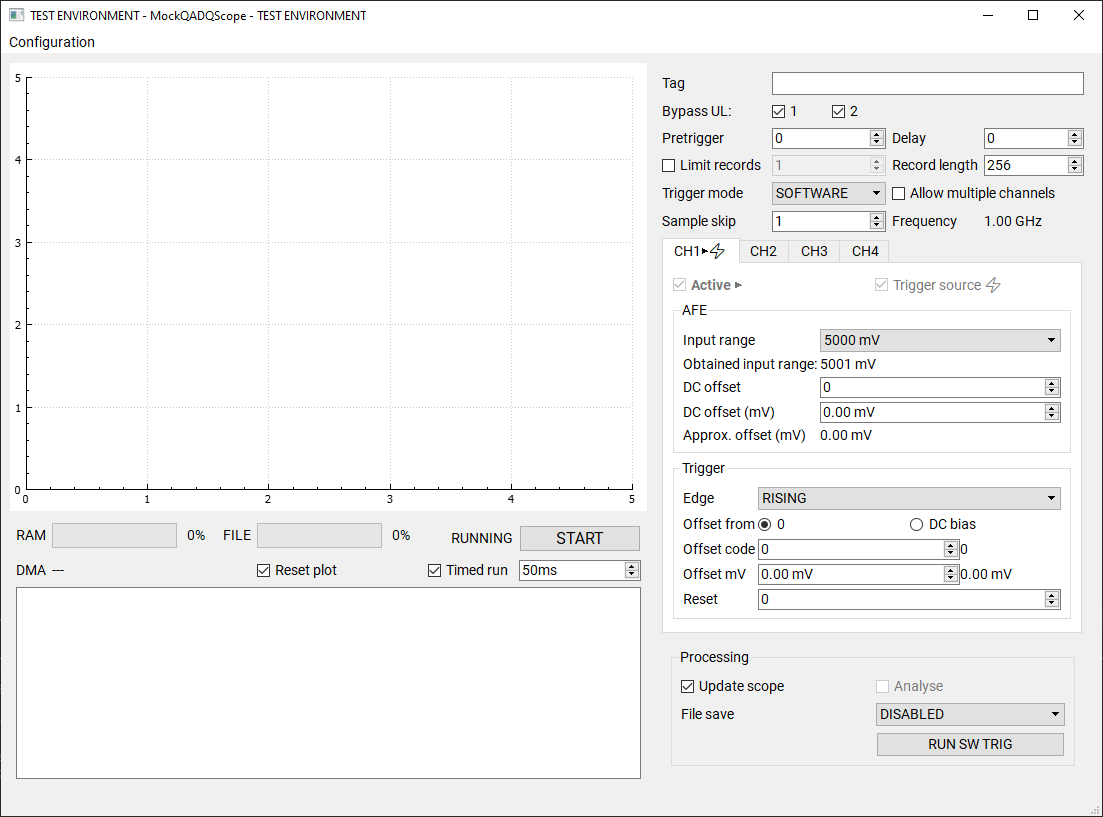
\includegraphics[width=\linewidth]{media/qtadqscope_v2.png}
  \caption{First major revision of the software application for acquisition}
  \label{fig:qtadqscope_v2} 
\end{figure}
\begin{figure}[H]
  \centering
  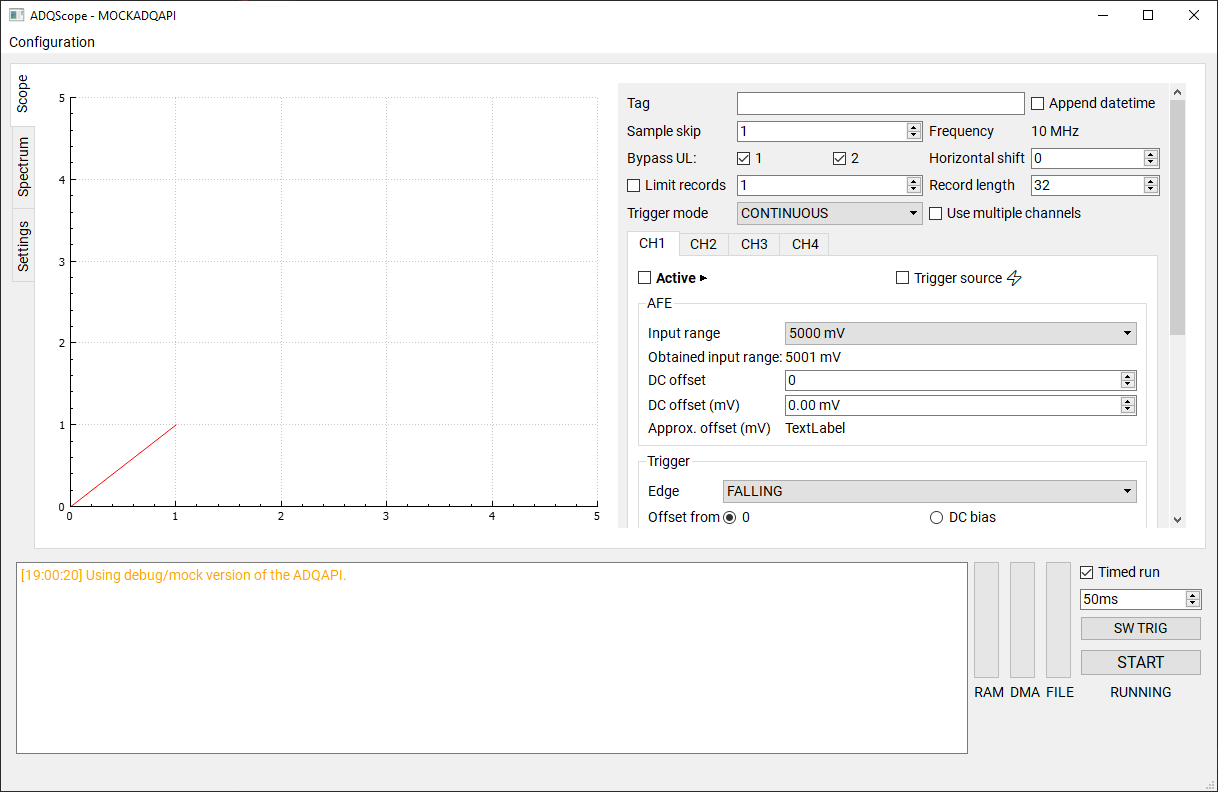
\includegraphics[width=\linewidth]{media/qtadqscope_v3.png}
  \caption{Current version of the software application for acquisition}
  \label{fig:qtadqscope_v3} 
\end{figure}
\subsubsection{Multi-threaded data transfer}

The primary thread of the software application
is used for UI display and general tasks like 
loading and saving configurations. Secondary threads
are spawned to control data acquisition and archival.
The proper operation of the worker threads
is crucial in maintaining a high data throughput.


The acquisition application was initially developed with 
the use of ADQAPI library in version 55575. That version
requires users to handle buffer processing and split the incoming
raw data into records with a custom built coroutine. \autoref{fig:adqapi_old_process}
shows the data path in version 55575. 

\begin{figure}[H]
  \centering
  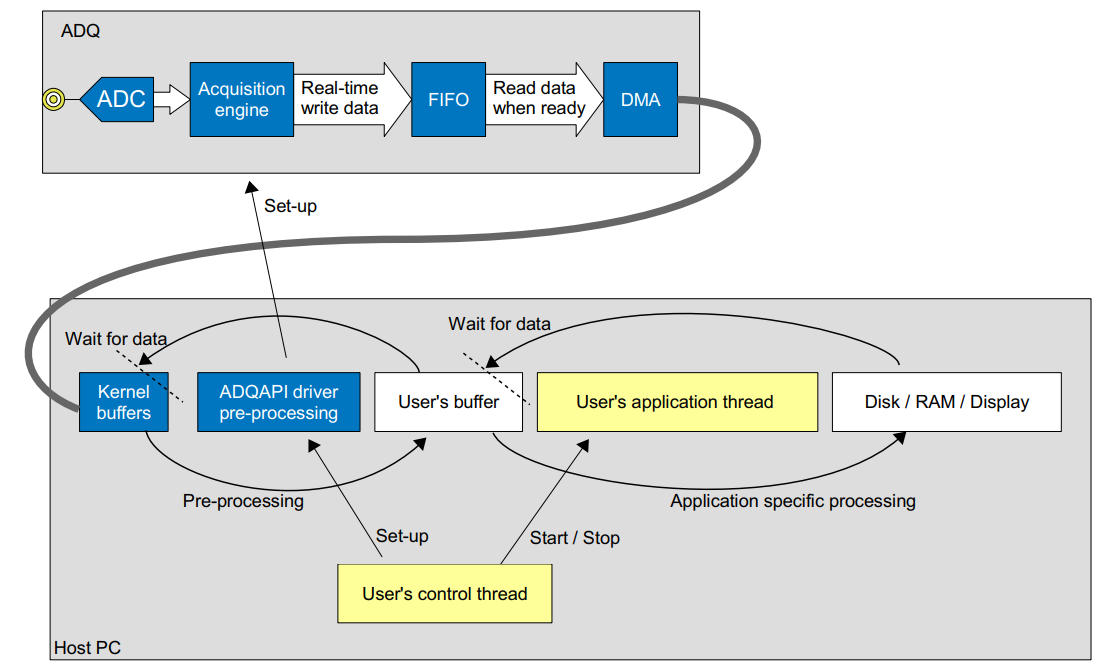
\includegraphics[width=\linewidth]{media/adqapi_old_process.png}
  \caption{Buffer transfer in ADQAPI v55575\cite{adq14_manual}}
  \label{fig:adqapi_old_process} 
\end{figure}

\autoref{fig:threads_in_old_app} shows the software acquisition pipeline in version 55575.
The maximum size of DMA buffers is limited, so as a first
step their contents is copied to another address in the PC's RAM 
to free their underlying memory.
This is done periodically in a separate worker thread.
As a DMA buffer becomes filled the worker locks one semaphore, reads its value
and copies the DMA buffer to a RAM buffer pointed to by the polled semaphore value.


Another thread polls the semaphores to get the number of filled buffers.
If a filled buffer is present it is read and processed. 
Each buffer contains a page with multiple records and their headers (metadata).
The records must be split based on the headers or a predefined configuration.
Each record is then passed on to further modules. Writing records to disk
is done in the same thread. If the records are to be displayed on screen
they must be sent over to the primary UI thread. 
Once a buffer is considered processed, the appropriate semaphore is incremented
to indicate that the buffer can be reused for writing.

\begin{figure}[H]
  \centering
  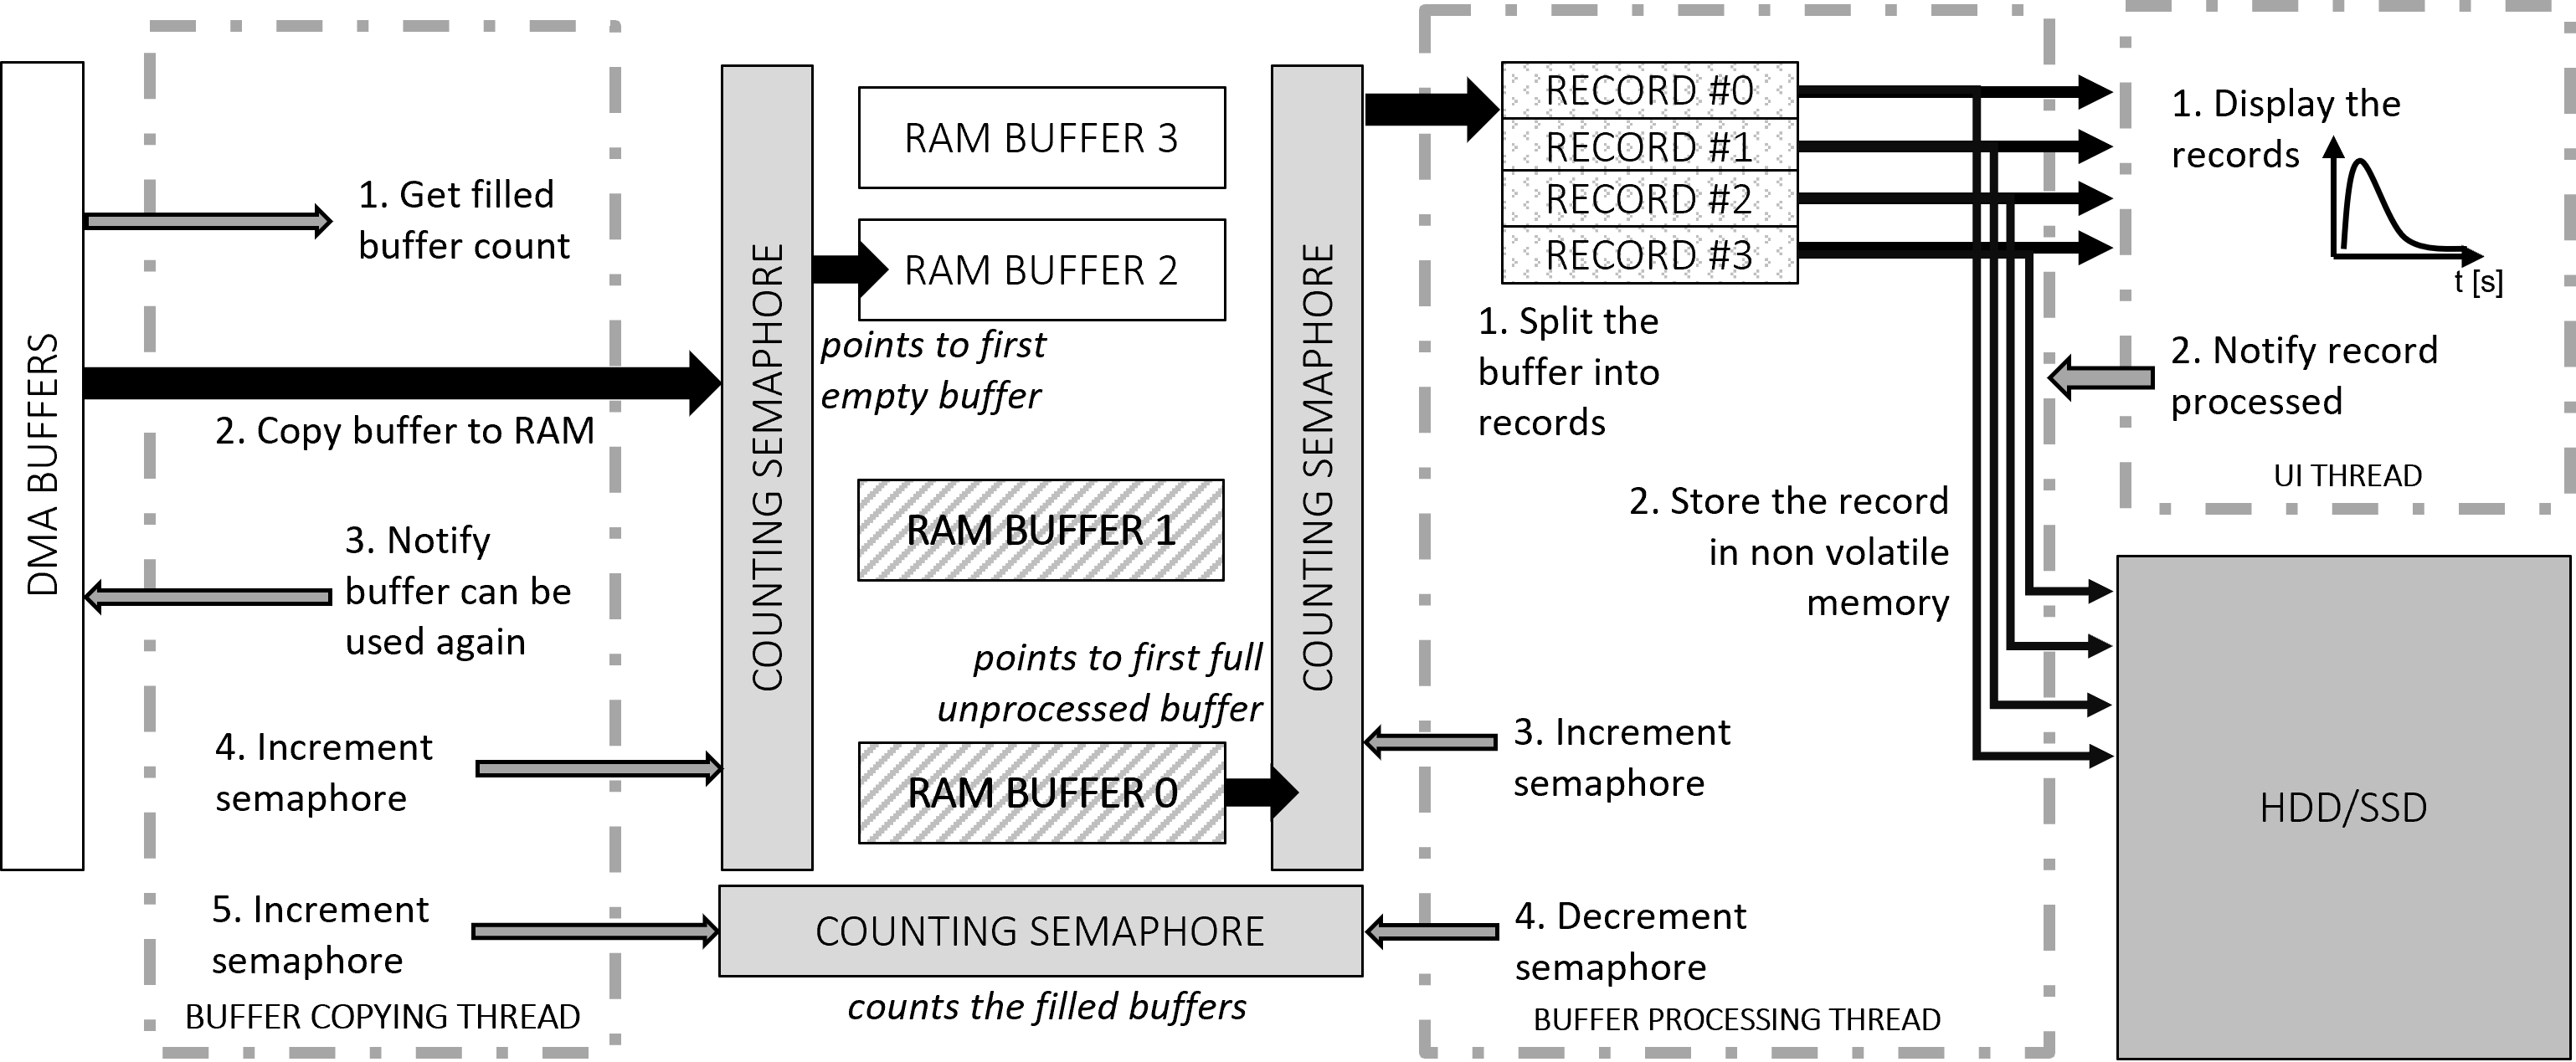
\includegraphics[width=\linewidth]{media/threads_in_old_app.png}
  \caption{Threads in the acquisition app with ADQAPI v55575}
  \label{fig:threads_in_old_app} 
\end{figure}

Plotting signals in real time is a bottleneck in the system. With a sufficiently fast
SSD drive the records can be reliably processed at a rate of up to a 1 GB/s.
The display feature, relies on a third-party library QCustomPlot which requires
the signed short integer samples output by ADQAPI
to be converted to a QVector of QDoubles (Qt5 wrappers over std::vector and double).
With as much as a few thousands of samples in each record, this is a costly operation that,
combined with the thread synchronization limits the maximum throughput to around 80 MB/s.
The scope is thus an optional feature intended for setup and debugging.


During the development of the application a new version of the ADQAPI library
was released to customers. The primary feature of ADQAPI in version 61716,
is a simplification of the buffer processing routine. The buffer copying thread
is now provided by the library. Instead of operating on raw DMA buffers,
users can choose to use the more abstract interface and work with already
split record buffers. In testing the abstraction layer was found to offer 80-90\% 
of the original performance, with the added benefit of removing a few bugs.
The new interface was implemented in the software application going forward.
\autoref{fig:threads_in_new_app} outlines the processing routine used in the more recent
version of the application.

\begin{figure}[H]
  \centering
  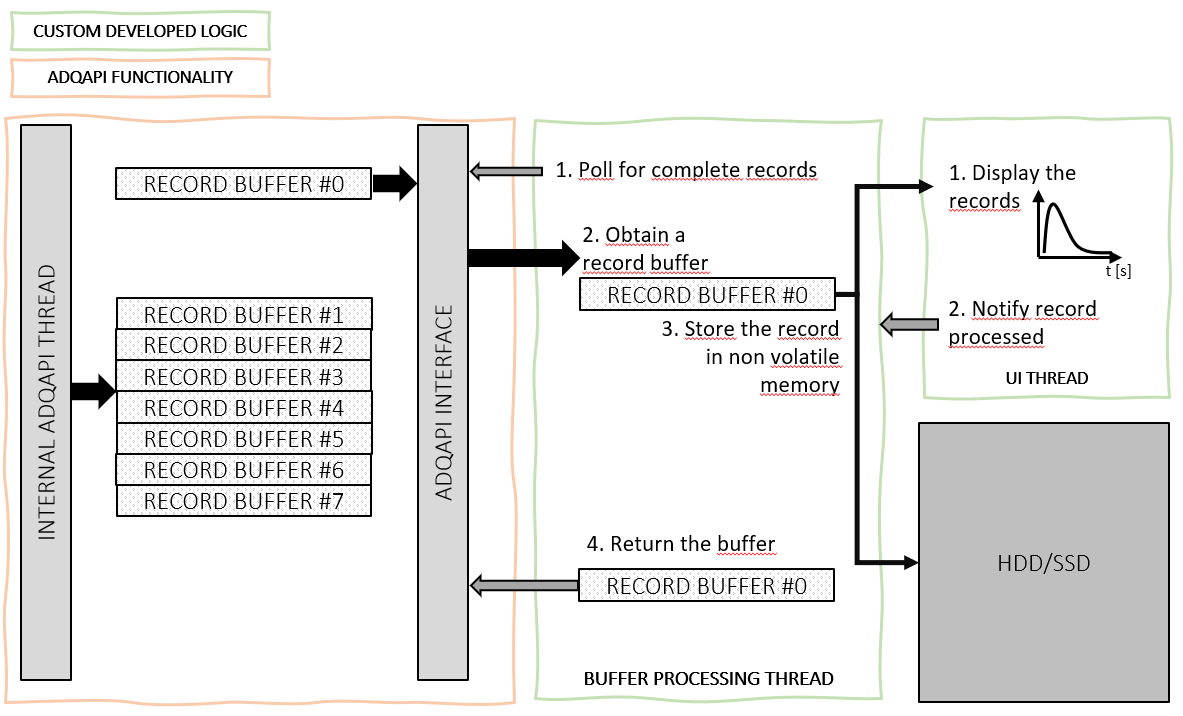
\includegraphics[width=\linewidth]{media/threads_in_new_app.png}
  \caption{Threads in the acquisition app with ADQAPI v61716}
  \label{fig:threads_in_new_app} 
\end{figure}

\subsubsection{Processing routine optimization}

A few other improvements were made to the processing routine over time.
The ADQAPI library is not thread safe. Nearly all function calls
must be done from a single synchronized thread. Accessing critical features
of the digitizer from two threads at once can crash the system.
In initial versions of the application thread safety was achieved
with a QMutex (Qt5 wrapper around std::mutex). A wrapper around the ADQAPI object
would lock the mutex before every function call. This approach enabled
the digitizer parameters to be accessed at any time, even during an acquisition.


With little input from the user the application would mostly perform
uncontested locks, which incur only a small overhead to the function calls.
The occasional contested locks could, however,
potentially cause a noticeable drop in performance.
To prevent that, the application was refactored to disable dynamic changes
to the digitizer during an acquisition. With that done, the mutex was removed
and the digitizer now exposed only a handful thread-safe methods for
starting, stopping and configuring acquisitions.
This change granted a small performance improvement of between 2-4\%
in the average throughput.


The current multithreading system relies on the use of QThreads and QObjects.
The QThread class is an interface built on top of C++ threads that 
works together with the Qt framework event queues.
In the application a worker object
that inherits from QObject is moved to a secondary QThread,
where it lives within an event loop.
This abstraction introduces an overhead when compared
to standard C++ threads, but greatly shortens the development time.
A version with a more optimized critical section is currently being developed.
Its performance will be measured once finished.

\subsubsection{Write speed optimization}

Additional upgrades were made to the disk write call itself. 
With a large amount of calls, each writing a small buffer, a drop in performance 
can be observable, when compared to lower level functions. Generally, writing 
longer chunks of data grants better performance. A simple test was performed
on the host PC to verify these facts. A series of writes was performed 
and their average write speed was noted. 
Writes were done in chunks, the size of which was changed in between tests.
\autoref{fig:chunk_bench} shows the results of this benchmark.


Initially the processing thread relied on calls to \lstinline{std::fstream::write()}.
Using \lstinline{std::fstream} introduces some abstraction over direct system calls.
The magnitude of the performance drop caused by write calls can differ 
depending on the implementation of the standard library and the computer's hardware.
To get the best possible performance the application has to be built
in release mode with the highest compiler optimization.


Typically writes are buffered, meaning that consecutive calls to a write function
actually flush to the storage medium after some buffer is filled. Until that 
the content of each write is copied over to the buffer.
Buffering can be disabled but in almost all use scenarios it causes
a massive performance drop. Fine tuning the buffer's size 
to a specific hardware and use case can lead to considerable write speed gains.


To find the best approach for the processing application, a series of simple 
write speed benchmarks were performed for varying writing methods. 
\lstinline{std::fstream} was used as the baseline and compared
to using \lstinline{FILE*} pointers with different buffer settings,
including non-buffered writes. UNIX file descriptors were also tested,
but caused up to an 80\% drop in performance, due to the lack of buffering.

  \begin{figure}[H]
    \centering
    \begin{minipage}{.45\textwidth}
      \centering
      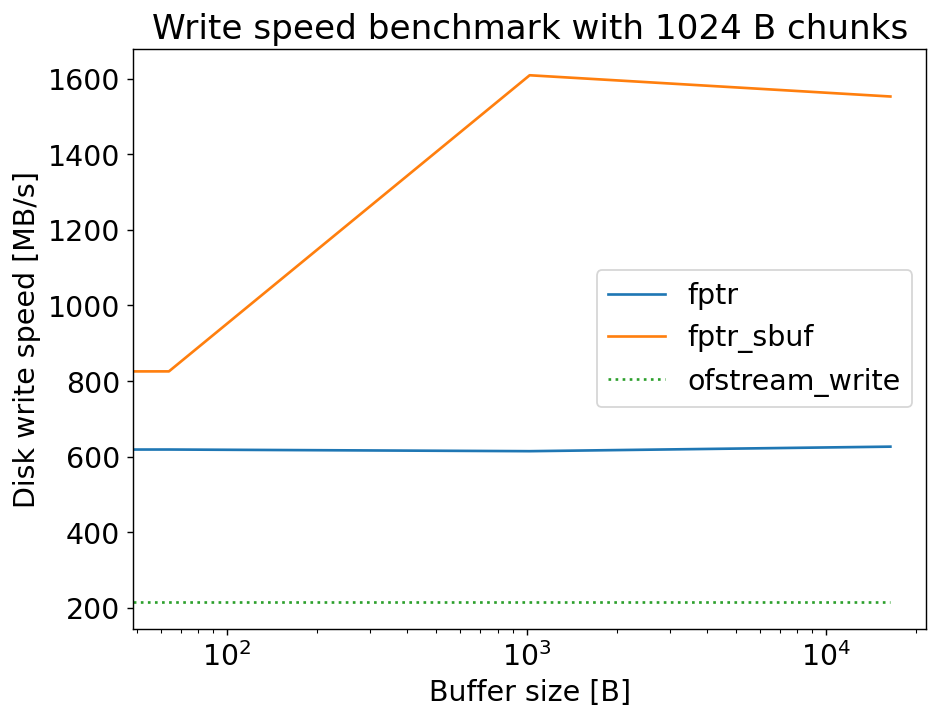
\includegraphics[width=\linewidth]{media/write_bench_1024.png}
      \caption{Write speed benchmark with a chunk size of 1024 bytes}
      \label{fig:write_bench_1024}
    \end{minipage}%
    \hfill
    \begin{minipage}{.45\textwidth}
      \centering
      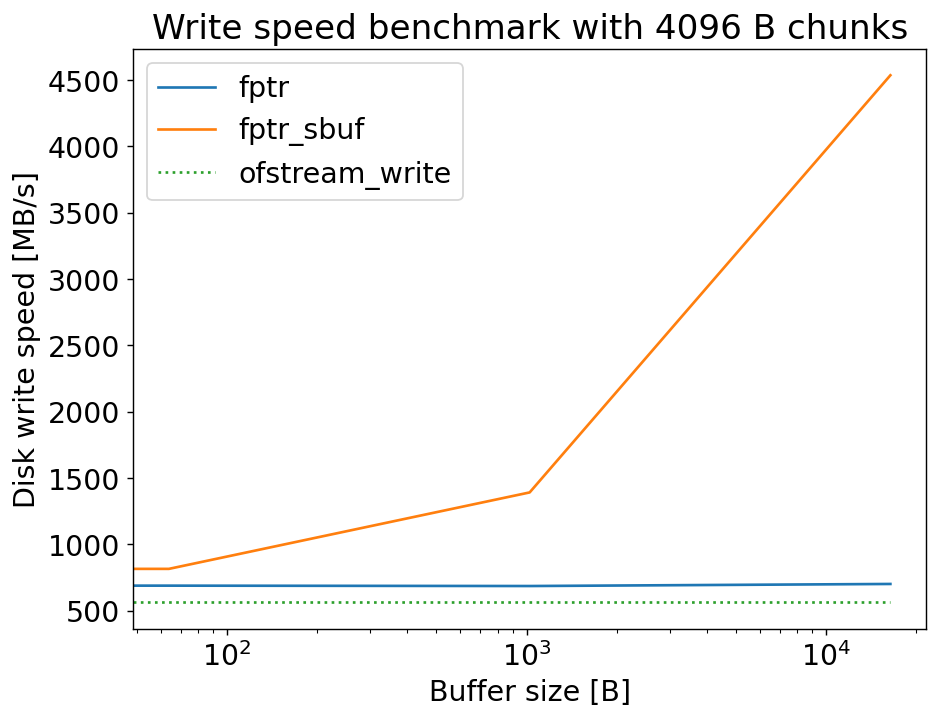
\includegraphics[width=\linewidth]{media/write_bench_4096.png}
      \caption{Write speed benchmark with a chunk size of 4096 bytes}
      \label{fig:write_bench_4096}
    \end{minipage}
  \end{figure}


  \begin{figure}[H]
    \centering
    \begin{minipage}{.45\textwidth}
      \centering
      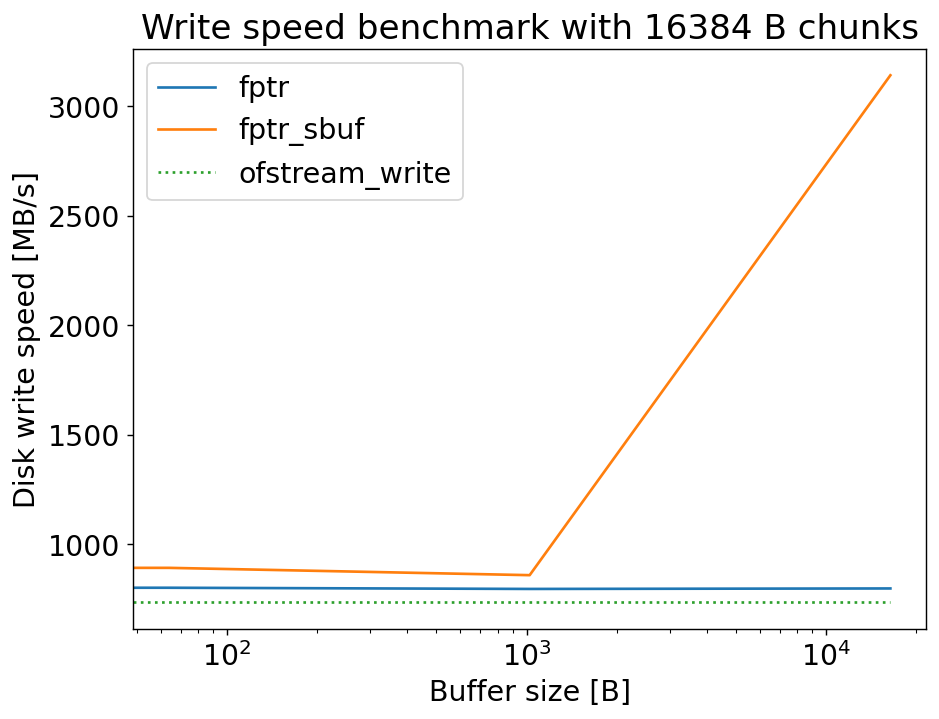
\includegraphics[width=\linewidth]{media/write_bench_16384.png}
      \caption{Write speed benchmark with a chunk size of 16384 bytes}
      \label{fig:write_bench_16384}
    \end{minipage}%
    \hfill
    \begin{minipage}{.45\textwidth}
      \centering
      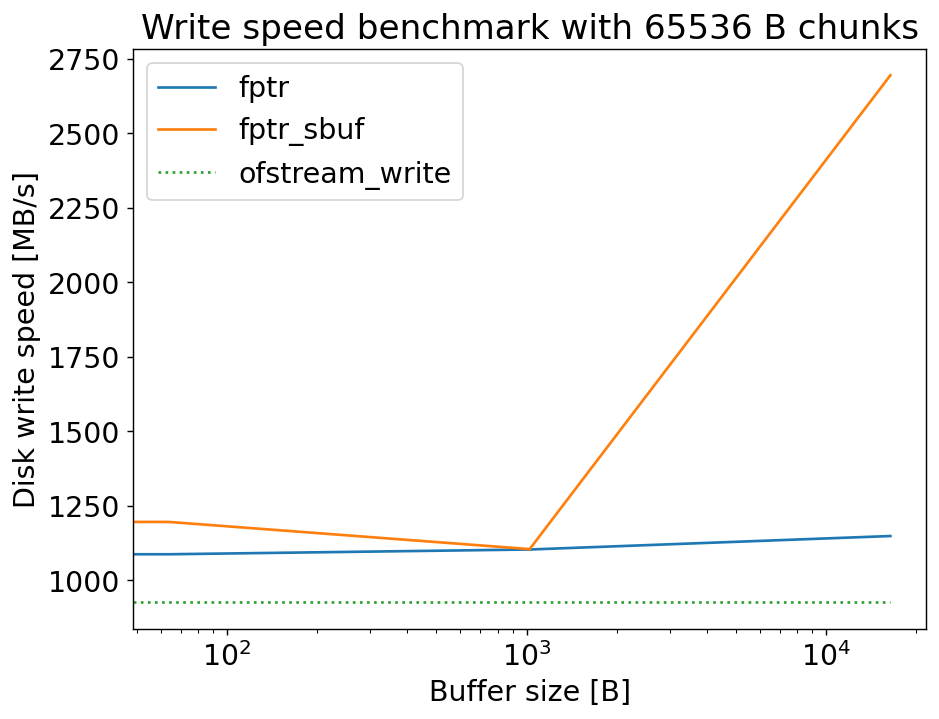
\includegraphics[width=\linewidth]{media/write_bench_65536.png}
      \caption{Write speed benchmark with a chunk size of 65536 bytes}
      \label{fig:write_bench_65536}
    \end{minipage}
  \end{figure}

  \begin{figure}[H]
    \centering
    \begin{minipage}{.45\textwidth}
      \centering
      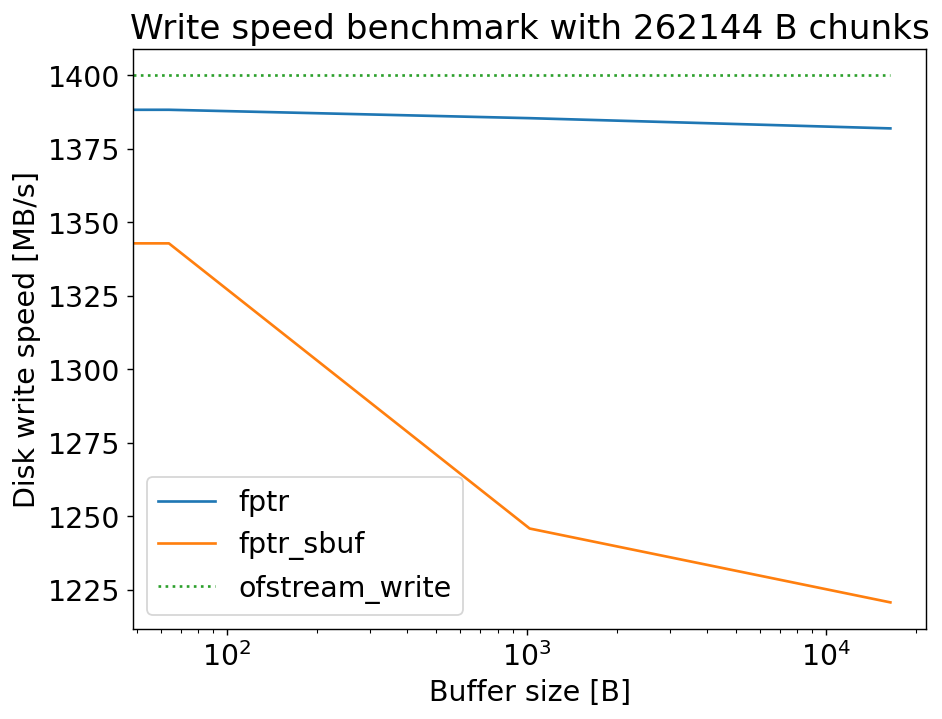
\includegraphics[width=\linewidth]{media/write_bench_262144.png}
      \caption{Write speed benchmark with a chunk size of 262144 bytes}
      \label{fig:write_bench_262144}
    \end{minipage}%
    \hfill
    \begin{minipage}{.45\textwidth}
      \centering
      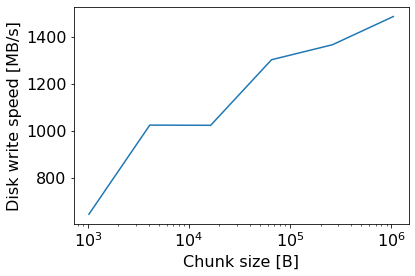
\includegraphics[width=\linewidth]{media/chunk_bench.png}
      \caption{Average write speed as a funciton of the chunk size}
      \label{fig:chunk_bench}
    \end{minipage}
  \end{figure}


The tests (\autoref{fig:write_bench_1024} - \autoref{fig:write_bench_262144})
indicate that the highest write speeds were obtained with
raw \lstinline{FILE*} pointers and user-controlled buffers (fptr\_sbuf) tuned
to the PC's SSD. In best conditions a threefold improvement
over default \lstinline{std::fstream} configuration was observed.
Letting the standard library manage the buffer
granted a stable improvement of up to 10\% in average write speed.
An equivalent drop was noticed when the size of the
chunks exceeded the size of buffers. For the time being the application 
was modified to use \lstinline{FILE*} based calls.


\newpage
\section{Conclusions}

This work described the design of 
a high-speed digital signal processing system for nuclear pulses
based on Field Programmable Gate Arrays.
Considerations and test results regarding real-time pulse detection, processing, 
multi-threaded acquisition systems and data transfer were presented.


A group of detection and shaping filters 
most commonly employed in Hard X-Ray Spectroscopy was compared.
The filters were first compared in research literature
and then implemented in both software and hardware to verify the results. 
Simulations were ran with different 
configurations to find the best algorithm to use in plasma diagnostics. With this
information the designs were implemented in a Field Programmable Gate Array
and interfaced with an Analog to Digital Converter sampling with a gigasample frequency.


While some digital filters perform substantially better than others
they come with different drawbacks. Fine-tuned algorithms like the trapezoidal filter
offer better accuracy than simple methods like the boxcar. The cost of this
increased accuracy is usually higher system complexity and lesser universality. 
Reduction of pile-up effects is one of the most important features of 
both detection and shaping algorithms.


Field Programmable Gate Arrays offer advantages over both 
ASICs and CPUs. In digital signal processing they offer greater parallelism
than CPUs, and much better reconfigurability when compared to ASICs. 
This makes them a perfect choice for highly experimental systems, like tokamaks.
With FPGAs changes to filters and algorithms can be introduced remotely and
can involve near complete rewrites of the underlying firmware.
On the other hand, although the devices allow for great performance gains, 
they often require complex algorithm pipelining in implementation. 
Additionally, the typical development time is longer than with CPUs.


Maintaining a high data throughput in digital signal processing systems
is a complicated task, that requires high optimization at multiple levels.
Internal buffers of the digitizer must be regularly transferred to the host PC.
The host PC must be capable of processing them at speeds comparable to their appearance.
This requires the use of multiprocessing.
Threaded applications come with a much greater amount of risk
and require a lot of optimization and debugging
when it comes to their routines and synchronization mechanisms.
Any software, hardware or firmware bottlenecks cause buffers to fill, 
which in turn greatly increase the likelihood of data loss.

\subsection{Further problems and research}

Despite a successful implementation of the system at hand, 
many problems that a similar setup will have to face
if used at ITER remain yet to be solved.
Pile-ups still pose a significant threat to the currently used processing algorithms. 
Some prototypes for rejection
were developed but their performance was not yet properly tested in firmware
due to time and resource constraints of this work.


The tests done on the constructed HXRM setup described here
involved only well-formed exponential pulses.
In ITER, the light attenuation from the fiber optic interface
will cause the pulse shapes to divert from exponential curves.
It is possible, that entirely different detection and shaping
algorithms will have to be developed for the new scenario. 


Apart from the functional upgrades, other minor system improvements are planned
in the near future. The critical section of the processing threads
is still in the process of being optimized. The UI is currently 
being reworked to provide a more intuitive experience. 
Some changes are planned to the firmware user registers, to produce
a more universal and easier to configure interface.



\newpage
%	BIBLIOGRAPHY
\printbibliography

\end{document}